%!TEX program = xelatex

% Name           : hsrm-beamer-minimal.sty
% Author         : Benjamin Weiss (benjamin.weiss@kreatiefton.de)
% Version        : 0.2
% Created on     : 08.05.2013
% Last Edited on : 24.03.2014
% Copyright      : Copyright (c) 2013 by Benjamin Weiss. All rights reserved.
% License        : This file may be distributed and/or modified under the
%                  GNU Public License.
% Description    : HSRM beamer theme minimal example.

\documentclass[usepdftitle=false]{beamer}

\usepackage[main=english,german]{babel}
\newcommand\Fontvi{\fontsize{6}{7.2}\selectfont}
\usetheme{hsrm}
\usepackage{graphicx}
\usepackage{subfigure}
\usepackage{amsbsy}
\usepackage{amssymb}
\usepackage{amsmath}
\usepackage{tabularx}
\usepackage{booktabs}
%\usepackage{floatrow}
%\usepackage{multirow}
%\usepackage{multicol}
\usepackage{enumerate}
\setbeamerfont{caption}{size=\scriptsize
}%\floatsetup[table]{capposition=top}
\newcommand{\matr}[1]{\mathbf{#1}}
\newenvironment{bsmallmatrix}
  {\left[\begin{smallmatrix}}
  {\end{smallmatrix}\right]}
\newenvironment{psmallmatrix}
  {\left\{\begin{smallmatrix}}
  {\end{smallmatrix}\right\}}
\newenvironment{psmatrix}
  {\left\{\begin{matrix}}
  {\end{matrix}\right\}}
\newcommand{\code}[1]{\texttt{#1}}
\newcolumntype{b}{X}
\newcolumntype{s}{>{\hsize=.5\hsize}X}
%\includeonlyframes{current}

\title{비선형 감쇠장치가 설치된 건축구조물의 내진 및 내풍 성능 평가를 위한 하이브리드 실험기법 및 가진시스템 설계}
\subtitle{Hybrid Testing Method and Excitation System Design for Seismic and Wind-resistance Performance Evaluation of Building Structures with Nonlinear Dampers}
\author{박은천}
\institute{단국대학교 건축대학 {\Medium 지도교수 : 민경원}}
\date{\today}

\begin{document}

\maketitle

\section*{Contents}
\begin{frame}
	\frametitle{Contents}
	\tableofcontents[hideallsubsections]
\end{frame}

\section{Introduction}

\begin{frame}{Introduction}
\begin{figure}[ht]
\centering
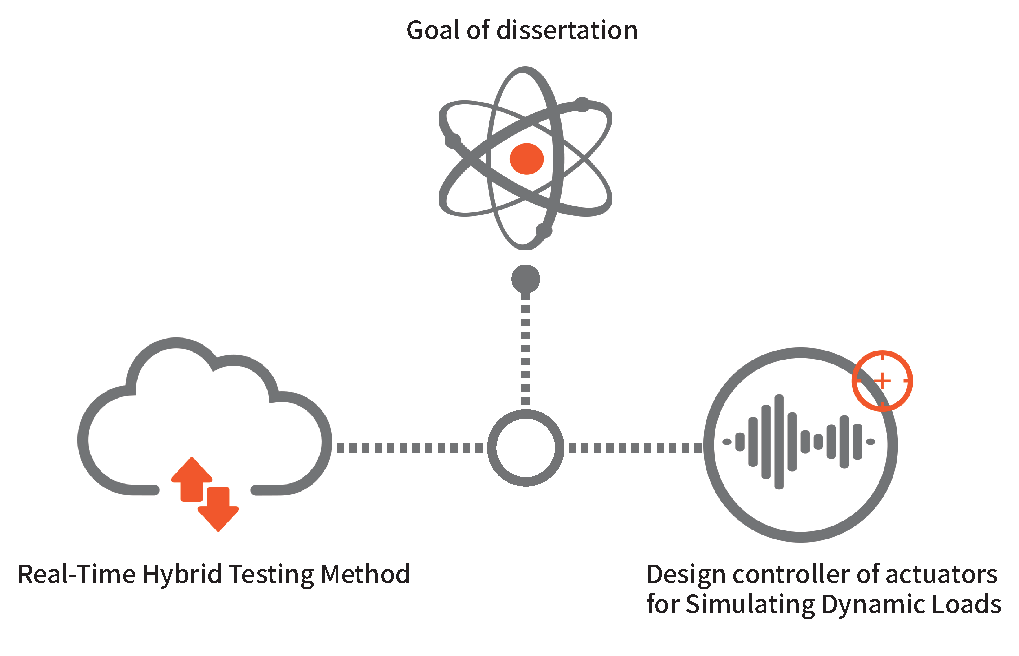
\includegraphics[width=1\textwidth] {figure/beamer-1.eps}
\end{figure}
\end{frame}

\begin{frame}{Introduction}
\begin{figure}[ht]
\centering
\includegraphics[width=1\textwidth] {figure/beamer-2.eps}
\end{figure}
\end{frame}

\begin{frame}{Introduction}
\begin{figure}[ht]
\centering
\includegraphics[width=1\textwidth] {figure/beamer-3.eps}
\end{figure}
\end{frame}

\begin{frame}{Introduction}
\begin{figure}[ht]
\centering
\includegraphics[width=1\textwidth] {figure/beamer-4.eps}
\end{figure}
\end{frame}

\begin{frame}{Introduction}
\begin{figure}[ht]
\centering
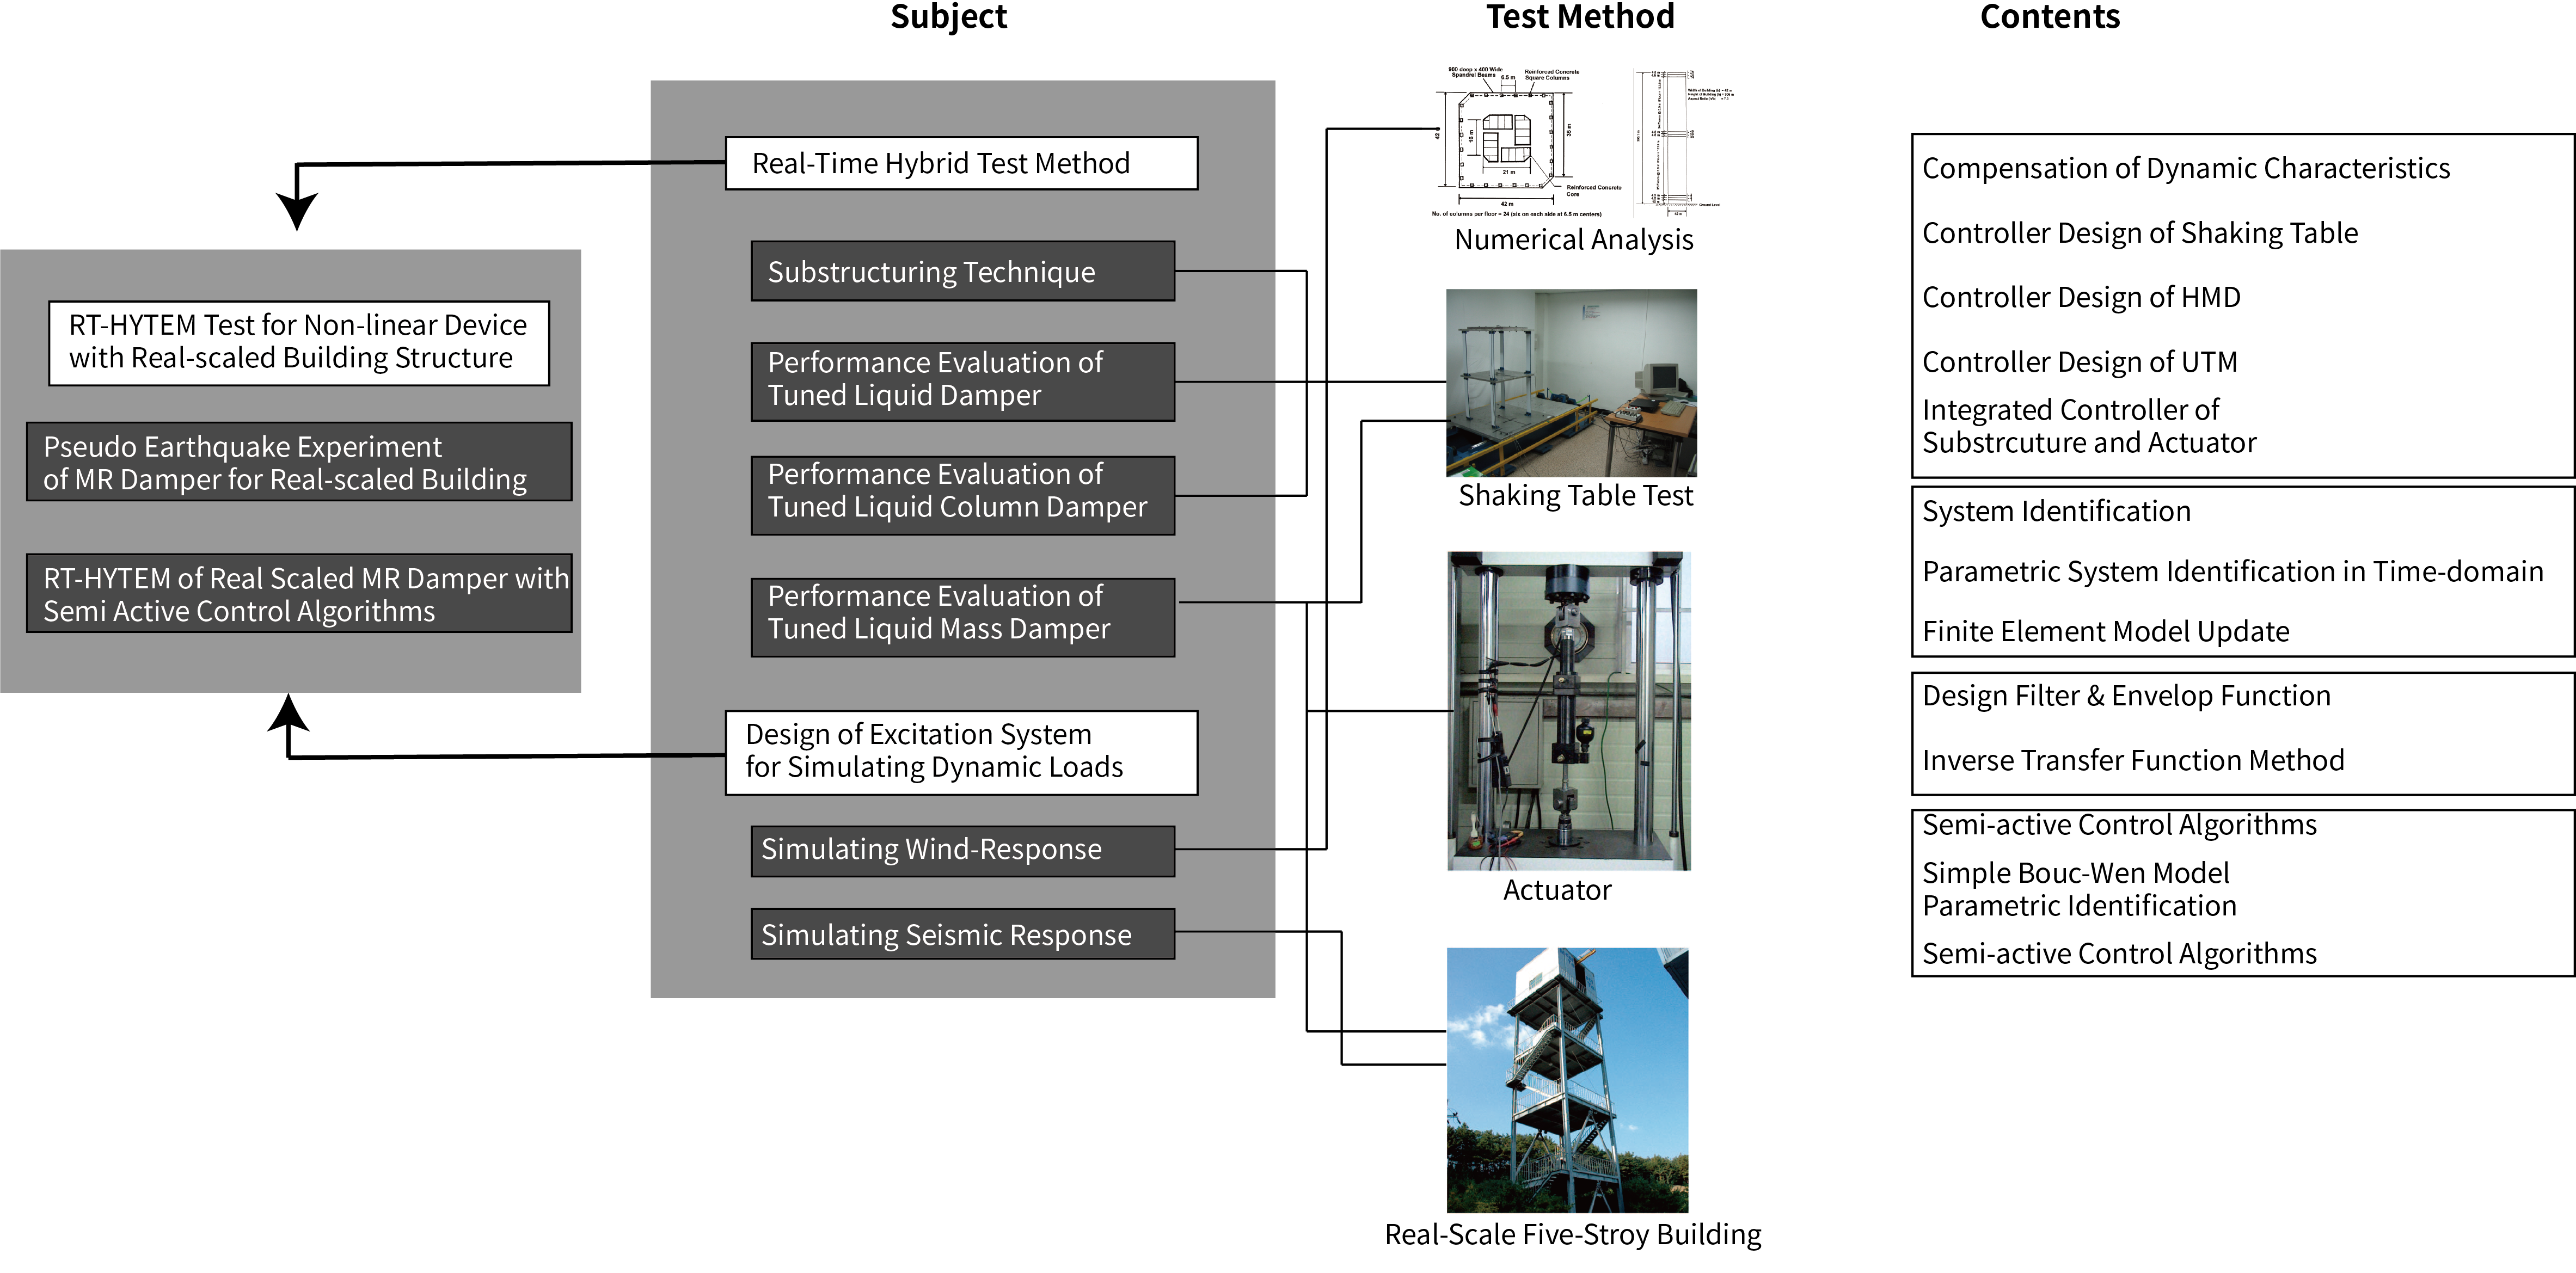
\includegraphics[width=1\textwidth] {figure/subject.eps}
\label{fig:subject}
\end{figure}
\end{frame}




\section{Publications}

\begin{frame}{International Journal (국제저널 SCI급)}
\Fontvi
\begin{itemize}
\item \textbf{Eunchurn Park}, Kyung-Won Min, Sung-Kyung Lee, Sang-Hyun Lee, Heon-Jae Lee, Seok-Jun Moon, Hyung-Jo Jung, “\textbf{Real-time Hybrid Test on a Semi-actively Controlled Building Structure Equipped with Full-scale MR Dampers}”, Journal of Intelligent Material Systems and Structures; 21(18):1831-1850. DOI:10.1177/1045389X10390253 · 2.17 Impact Factor
\item Heon-Jae Lee, Hyung-Jo Jung, Seok-Jun Moon, Sung-Kyung Lee, \textbf{Eun-Churn Park}, Kyung-Won Min, “\textbf{Experimental Investigation of MR Damper-based Semiactive Control Algorithms for Full-scale Five-story Steel Frame Building}”, Journal of Intelligent Material Systems and Structures; 21(10):1025-1037. DOI:10.1177/1045389X10374162 · 2.17 Impact Factor
\item Jae-Sung Heo, Sung-Kyung Lee, \textbf{Eunchurn Park}, Sang-Hyun Lee, Kyung-Won Min, Hongjin Kim, Jiseong Jo, Bong-Ho Cho, “\textbf{Performance test of a tuned liquid mass damper for reducing bidirectional responses of building structures}”, The Structural Design of Tall and Special Buildings; 18(7):789 - 805. DOI:10.1002/tal.486 · 0.83 Impact Factor
\item \textbf{Eun-Churn Park}, Sang-Hyun Lee, Kyung-Won Min, Lan Chung, Sung-Kyung Lee, Seung-Ho Cho, Eunjong Yu, Kyung-Soo Kang, “\textbf{Design of an actuator for simulating wind-induced response of a building structure}”, SMART STRUCTURES AND SYSTEMS; 4(1). DOI:10.12989/sss.2008.4.1.085 · 1.16 Impact Factor
\item Sung-Kyung Lee, \textbf{Eun Churn Park}, Kyung-Won Min, Ji-Hun Park, “\textbf{Real-time substructuring technique for the shaking table test of upper substructures}”, Engineering Structures; 29(9):2219-2232. DOI:10.1016/j.engstruct.2006.11.013 · 1.77 Impact Factor
\item Sung-Kyung Lee, \textbf{Eun Churn Park}, Kyung-Won Min, Sang-Hyun Lee, Ji-Hun Park, “\textbf{Experimental implementation of a building structure with a tuned liquid column damper based on the real-time hybrid testing method}”, Journal of Mechanical Science and Technology; 21(6):885-890. DOI:10.1007/BF03027063 · 0.70 Impact Factor
\item Sung-Kyung Lee, \textbf{Eun Churn Park}, Kyung-Won Min, Sang-Hyun Lee, Lan Chung, Ji-Hun Park, “ \textbf{Real-time hybrid shaking table testing method for the performance evaluation of a tuned liquid damper controlling seismic response of building structures}”, Journal of Sound and Vibration; DOI:10.1016/j.jsv.2006.12.006 · 1.86 Impact Factor
\end{itemize}
\end{frame}

\begin{frame}{Domestic Journal (국내저널 KCI등재)}
\Fontvi
\begin{itemize}
\item 민경원, 이성경, 박은천, “진동대실험에 의한 동조액체기둥감쇠기의 동적특성”, 한국소음진동공학회논문집 (Transactions of the Korean society for noise and vibration engineering) v.19 no.6 = no.147, pp.620 - 627, 2009, 1598-2785
\item 박은천, 이성경, 이헌재, 문석준, 정형조, 민경원, “대형 MR감쇠기가 설치된 건축구조물의 실시간 하이브리드 실험 및 준능동 알고리즘 적용”, 한국전산구조공학회논문집 (Journal of the computational structural engineering institute of Korea) v.21 no.5, pp.465 - 474, 2008, 1229-3059
\item 이성경, 민경원, 박은천, “TMD와 TLCD를 이용한 2방향 감쇠기의 동적특성”, 한국전산구조공학회논문집 (Journal of the computational structural engineering institute of Korea) v.21 no.6, pp.589 - 596, 2008, 1229-3059
\item 허재성, 이성경, 박은천, 이상현, 김홍진, 조지성, 조봉호, “실시간 하이브리드 진동대 실험법에 의한 양방향 TLMD의 진동제어 성능평가”, 한국소음진동공학회논문집 (Transactions of the Korean society for noise and vibration engineering) v.18 no.5 = no.134, pp.485 - 495, 2008, 1598-2785
\item 허재성, 박은천, 이상현, 이성경, 김홍진, 조봉호, 조지성, 김동영, 민경원, “건축구조물의 2방향 진동제어를 위한 동조액체질량감쇠기”, 한국소음진동공학회논문집 (Transactions of the Korean society for noise and vibration engineering) v.18 no.3 = no.132, pp.345 - 355, 2008, 1598-2785
\item 허재성, 박은천, 이성경, 이상현, 김홍진, 조지성, 조봉호, 주석준, 민경원, “실물크기 구조물에 설치된 동조액체질량감쇠기의 성능실험”, 한국전산구조공학회논문집 (Journal of the computational structural engineering institute of Korea) v.21 no.2, pp.161 - 168, 2008, 1229-3059
\item 윤경조, 박은천, 이헌재, 문석준, 민경원, 정형조, 이상현, “준능동 MR감쇠기가 설치된 실물크기 구조물의 분산제어 알고리즘 성능평가”, 한국소음진동공학회논문집 (Transactions of the Korean society for noise and vibration engineering) v.18 no.2 = no.131, pp.255 - 262, 2008, 1598-2785
\end{itemize}
\end{frame}

\begin{frame}{Domestic Journal (국내저널 KCI등재)}
\Fontvi
\begin{itemize}
\item 박은천, 이성경, 윤경조, 정희산, 이헌재, 최강민, 문석준, 정형조, 민경원, “실시간 하이브리드 실험법을 이용한 대형 MR감쇠기의 제진 성능평가”, 한국소음진동공학회논문집 (Transactions of the Korean society for noise and vibration engineering) v.18 no.1 = no.130, pp.131 - 138, 2008, 1598-2785
\item 박은천, 민경원, 정란, 강경수, 이상현, “건축구조물의 풍하중 구현 및 풍특성 평가를 위한 가진시스템 설계”, 한국전산구조공학회논문집 (Journal of the computational structural engineering institute of Korea) v.20 no.6, pp.769 - 778, 2007, 1229-3059
\item 이성경, 민경원, 박은천, “진동대를 이용한 구조물의 하이브리드 실험”, 대한건축학회논문집 (Journal of the architectural institute of Korea : Structure \& construction) / 구조계 v.22 no.5 = no.211, pp.57 - 63, 2006, 1226-9107
\item 이상현, 박은천, 윤경조, 이성경, 유은종, 민경원, 정란, 민정기, 김영찬, “실물 크기 구조물의 강제진동실험 및 지진응답 모사를 위한 HMD제어기 설계”, 한국지진공학회논문집 (Journal of the earthquake engineering society of Korea) v.10 no.6 = no.52, pp.103 - 114, 2006, 1226-525x
\item 이성경, 박은천, 이상현, 정란, 우성식, 민경원, “실시간 하이브리드 진동대 실험법을 이용한 TLD 제어성능의 실험적 검증”, 한국전산구조공학회논문집 (Journal of the computational structural engineering institute of Korea) v.19 no.4 = no.74, pp.419 - 427, 2006, 1229-3059
\end{itemize}
\end{frame}



\section{Hybrid Testing Method}
\begin{frame}{Hybrid Testing Method (Substructuring Technique)}
\begin{figure}[ht]
\centering
\subfigure{
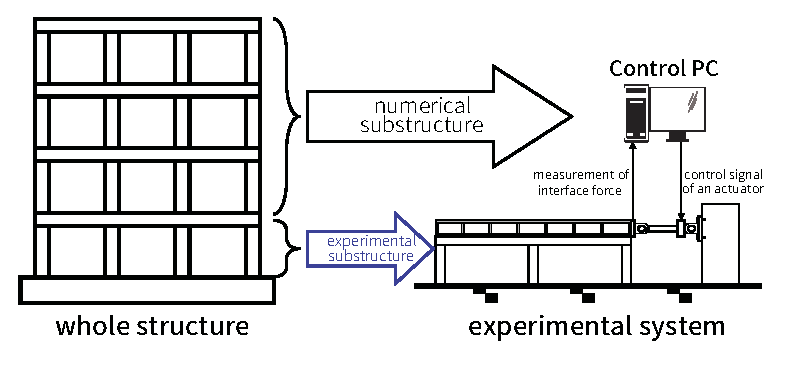
\includegraphics[width=0.5\textwidth] {figure/2_1a.eps}
}\hfill
\subfigure{
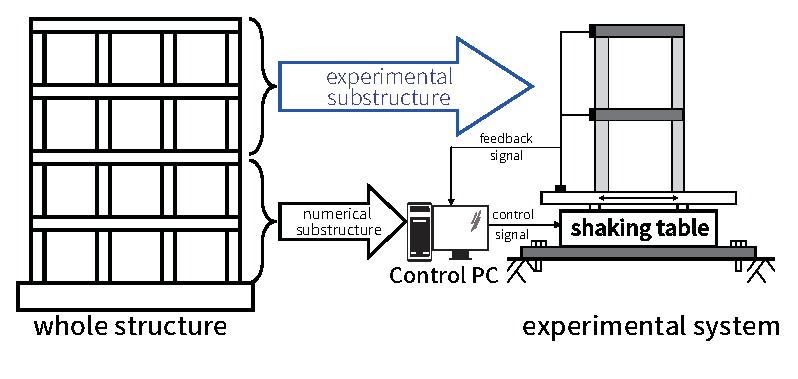
\includegraphics[width=0.5\textwidth] {figure/2_1b.eps}
}
\end{figure}
\end{frame}


\begin{frame}{Dynamic equilibrium in experimental structure}
\begin{figure}[ht]
\setcounter{subfigure}{0}
\centering\subfigure[Whole structure]{
   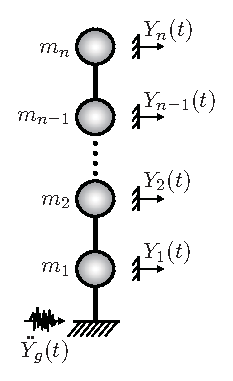
\includegraphics[width=0.2\textwidth] {figure/2-3a.eps}
   \label{fig:2-3a}
 }\hfill
 \subfigure[Separation of whole structure]{
   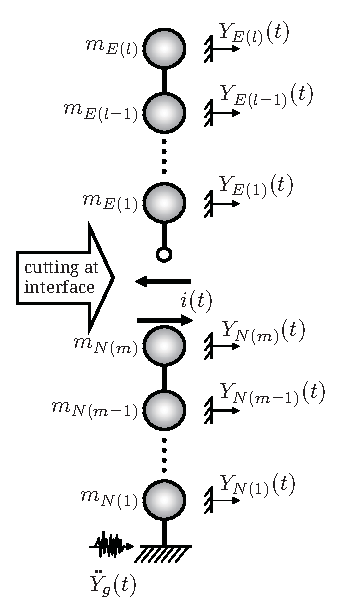
\includegraphics[width=0.3\textwidth] {figure/2-3b.eps}
   \label{fig:2-3b}
 }\hfill
 \subfigure[Experimental and numerical substructure]{
   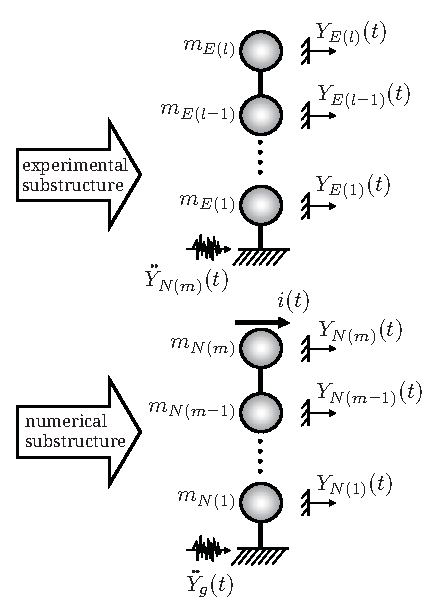
\includegraphics[width=0.4\textwidth] {figure/2-3c.eps}
   \label{fig:2-3c}
 }
\end{figure}
\end{frame}


\begin{frame}{Overall view of experimental system}
\begin{figure}[ht]
\centering
\includegraphics[width=1\textwidth] {figure/2-5.eps}
\end{figure}
\end{frame}


\begin{frame}{Schematic diagram of experimental system}
\begin{figure}[ht]
\centering
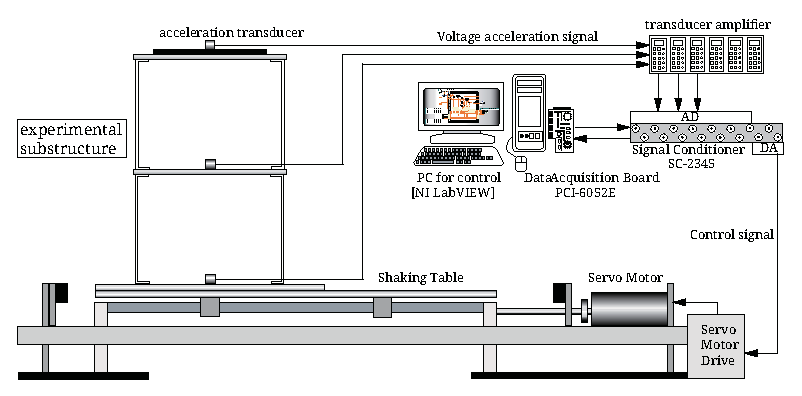
\includegraphics[width=1\textwidth] {figure/2-6.eps}
\end{figure}
\end{frame}

\begin{frame}{Flow chart of the experimental system controller}
\begin{figure}[ht]
\centering
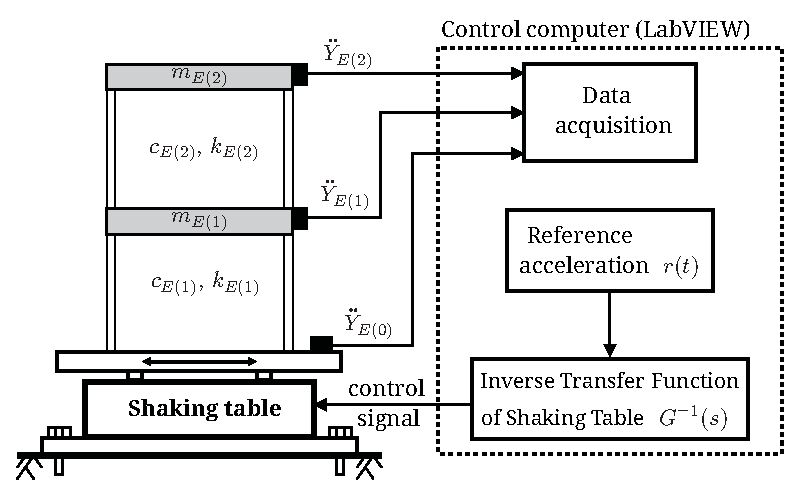
\includegraphics[width=1\textwidth] {figure/2-8.eps}
\end{figure}
\end{frame}


\begin{frame}{Interfacing Force}
\begin{align}
i(t)=&-m_{E(1)}\ddot{Y}_{E(1)}(t)-m_{E(2)}\ddot{Y}_{E(2)}(t) \label{eq:2-19} \\
\ddot{Y}_{N(3)}(t)=&-c_{N(3)}\left(\dot{Y}_{N(3)}-\dot{Y}_{N(2)}\right) -k_{N(3)}\left(Y_{N(3)}-Y_{N(2)}\right)+i(t) \label{eq:2-20}
\end{align}

\begin{figure}[ht]
\centering
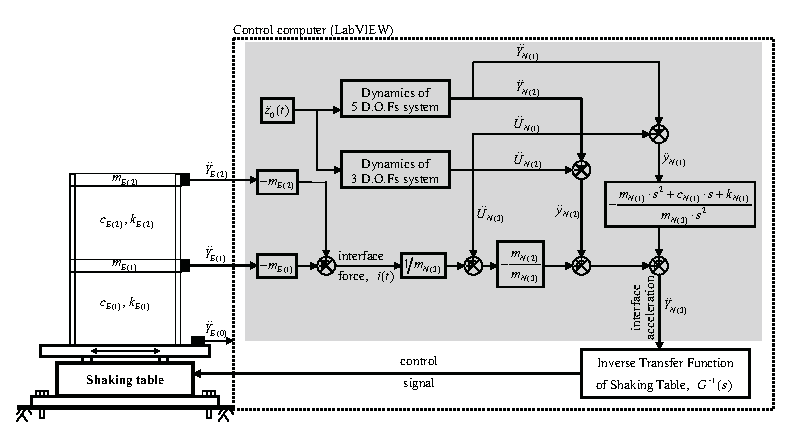
\includegraphics[width=0.8\textwidth] {figure/2-11.eps}
\end{figure}
\end{frame}


\begin{frame}{Comparisons of results}
\begin{figure}[ht]
\centering
\setcounter{subfigure}{0}
\subfigure[Time domain]{
   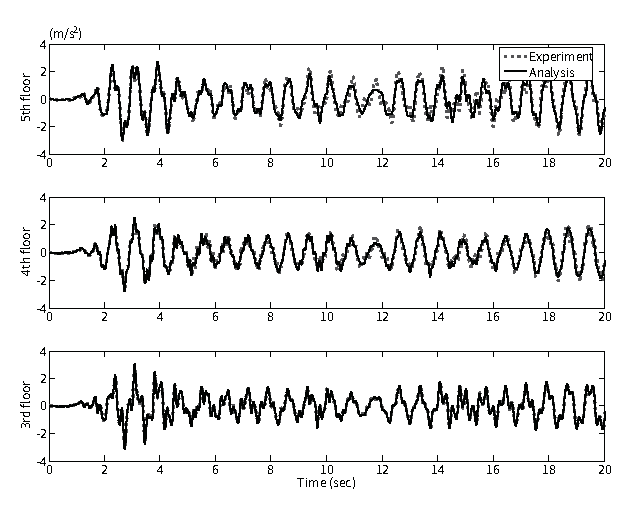
\includegraphics[width=0.4\textwidth] {figure/2-12a.eps}
   \label{fig:2-12a}
 }
 \subfigure[Frequency domain]{
   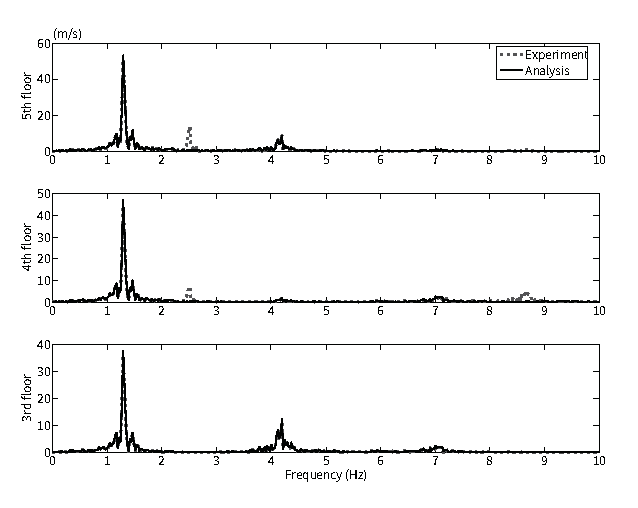
\includegraphics[width=0.4\textwidth] {figure/2-12b.eps}
   \label{fig:2-12b}
 }
%\caption{Comparisons of results measured from the experiment without feedback and those calculated from numerical analysis.}
\label{fig:2-12}
\end{figure}
\end{frame}

\begin{frame}{Spectrogram comparison of results}
\begin{figure}[ht]
\centering
\setcounter{subfigure}{0}
 \subfigure[experiment without feedback]{
   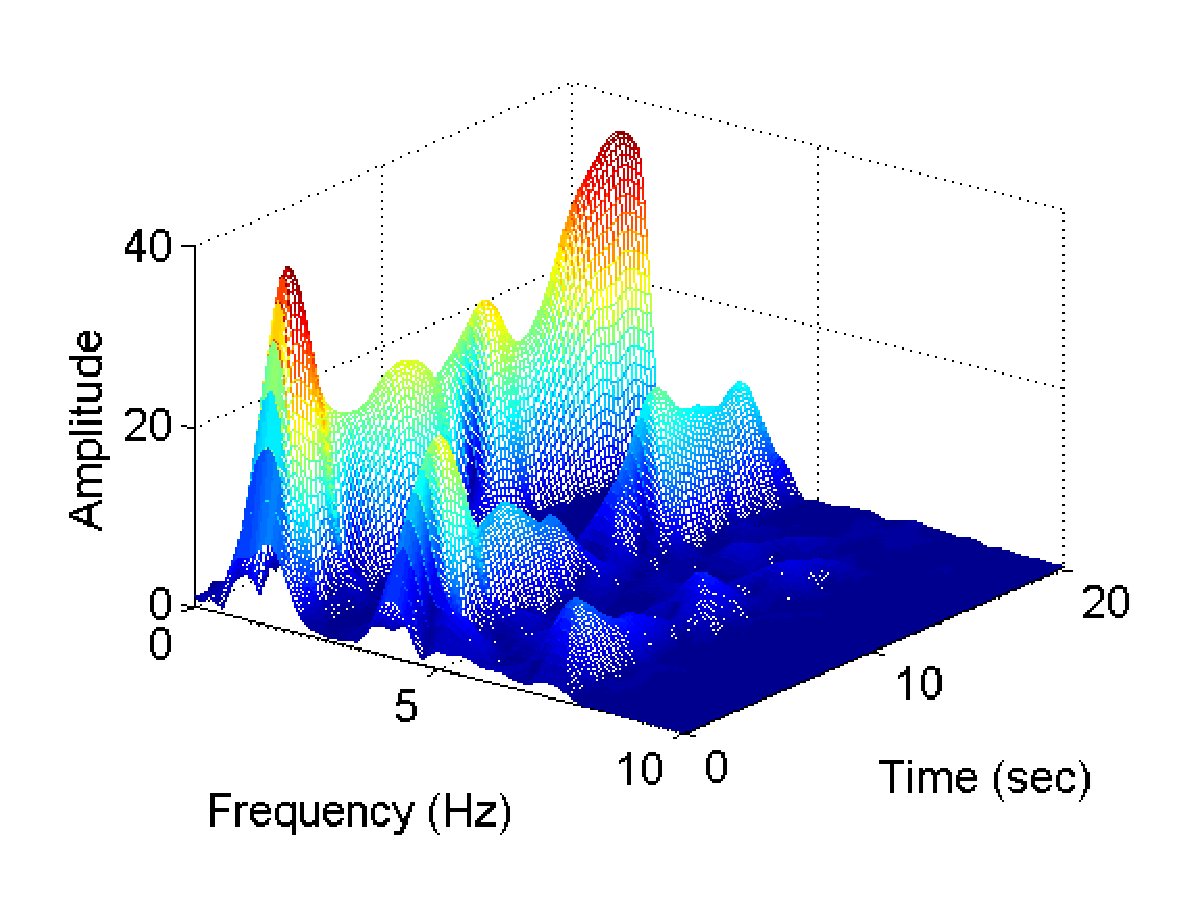
\includegraphics[width=0.35\textwidth] {figure/2-13a.eps}
   \label{fig:2-13a}
 }\hfill
 \subfigure[numerical analysis measured]{
   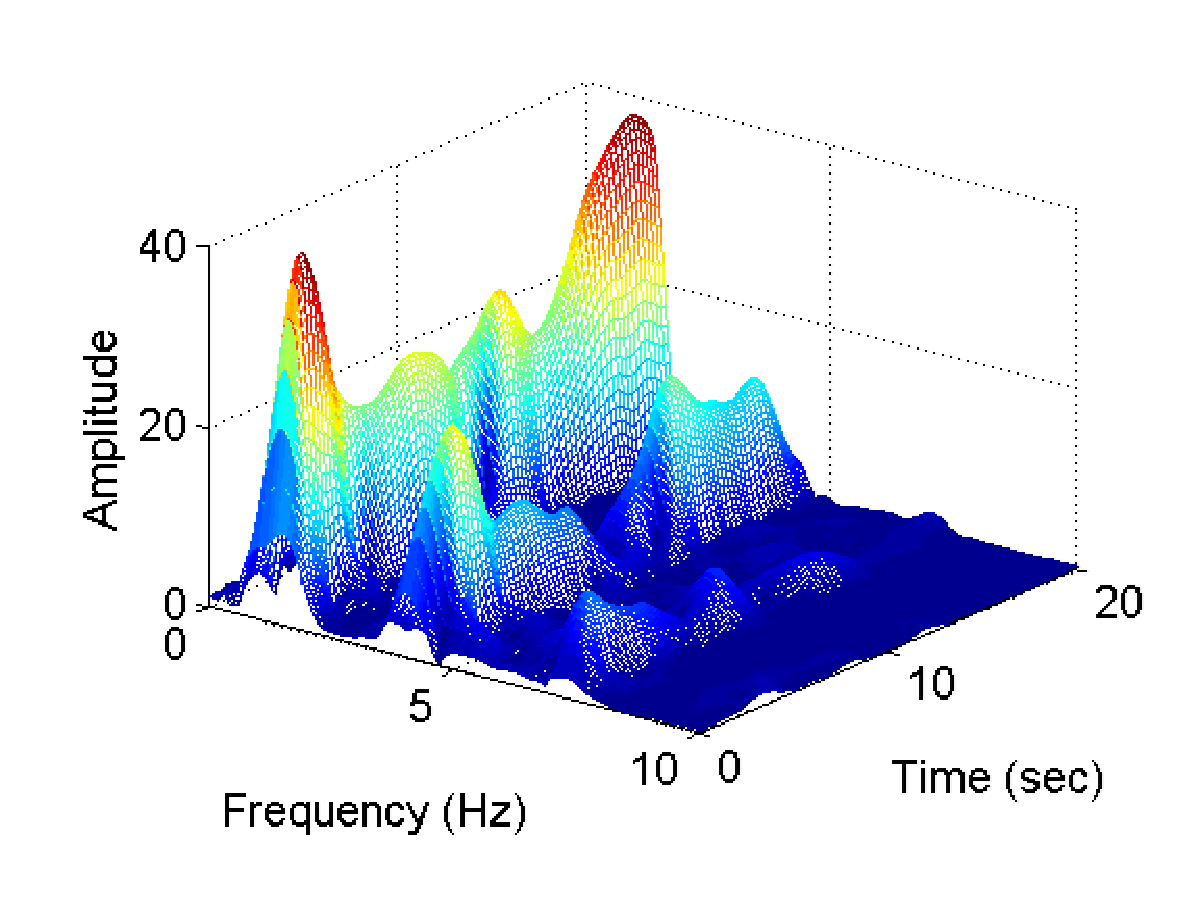
\includegraphics[width=0.35\textwidth] {figure/2-13b.eps}
   \label{fig:2-13b}
 }\\
 \subfigure[experiment without feedback]{
   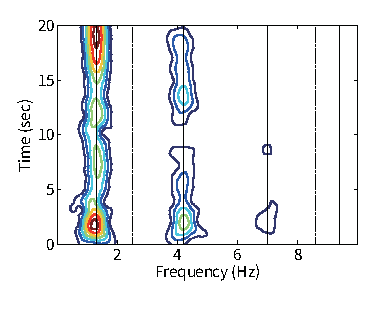
\includegraphics[width=0.35\textwidth] {figure/2-13c.eps}
   \label{fig:2-13c}
 }\hfill
 \subfigure[numerical analysis measured]{
   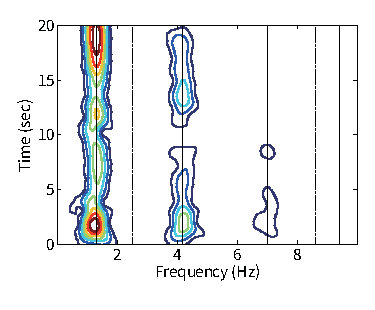
\includegraphics[width=0.35\textwidth] {figure/2-13d.eps}
   \label{fig:2-13d}
 }
\end{figure}
\end{frame}

\begin{frame}{Hybrid Testing for a TLD with Building Structure}
\begin{figure}[ht]
\centering
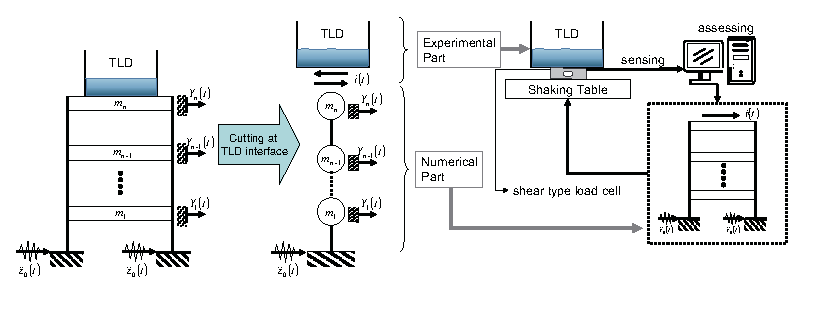
\includegraphics[width=1\textwidth] {figure/3-1.eps}
%\caption{Conceptual view of the real-time hybrid shaking table test}
%\label{fig:3-1}
\end{figure}
\end{frame}

\begin{frame}{Hybrid Testing for the Performance Evaluation of a TLD}
\begin{figure}[ht]
\centering
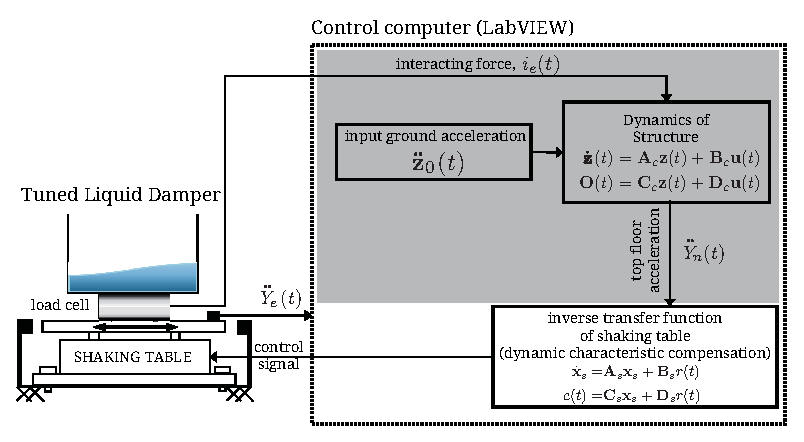
\includegraphics[width=1\textwidth] {figure/3-3.eps}
%\caption{Block diagram of the integrated controller for the real-time hybrid experimental system.}
\label{fig:3-3}
\end{figure}
\end{frame}

\begin{frame}{Hybrid Testing for the Performance Evaluation of a TLD}
\begin{figure}[!ht]
\centering
\setcounter{subfigure}{0}
\subfigure[Conventional shaking table test]{
   \includegraphics[width=0.45\textwidth] {figure/3-4a.eps}
   \label{fig:3-4a}
 }
 \subfigure[Real-time hybrid shaking table test]{
   \includegraphics[width=0.45\textwidth] {figure/3-4b.eps}
   \label{fig:3-4b}
 }
\end{figure}
\end{frame}


\begin{frame}{Hybrid Testing for the Performance Evaluation of a TLD}
\begin{figure}[!ht]
\centering
\setcounter{subfigure}{0}
 \subfigure[El Centro]{
   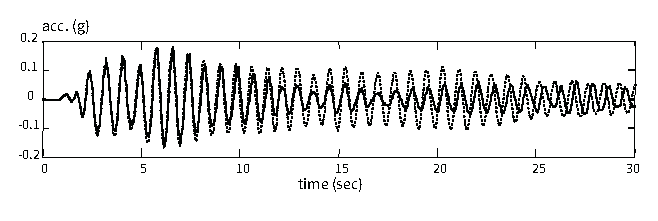
\includegraphics[width=0.4\textwidth] {figure/3-6a.eps}
   \label{fig:3-6a}
 }
 \subfigure[Hachinohe]{
   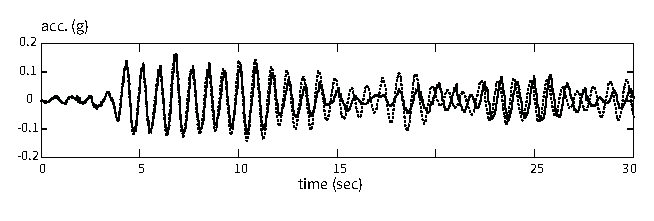
\includegraphics[width=0.4\textwidth] {figure/3-6b.eps}
   \label{fig:3-6b}
 }
 \subfigure[Mexico city]{
   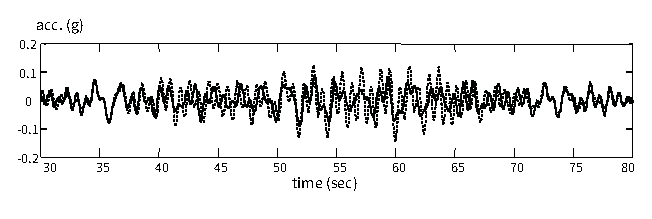
\includegraphics[width=0.4\textwidth] {figure/3-6c.eps}
   \label{fig:3-6c}
 }
 \subfigure[Northridge]{
   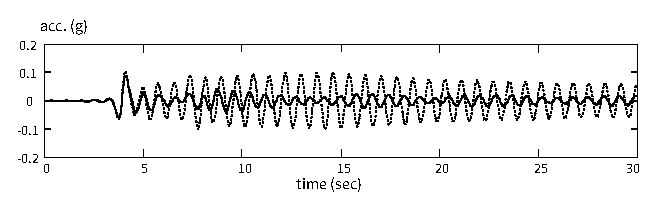
\includegraphics[width=0.4\textwidth] {figure/3-6d.eps}
   \label{fig:3-6d}
 }
%\caption{Structural acceleration in the time domain measured from the conventional shaking table test of TLD-structure interaction system (dotted line : without control, solid line : with control)}
\label{fig:3-6}
\end{figure}
dotted line : without control, solid line : with control

\end{frame}

\begin{frame}{Hybrid Testing for the Performance Evaluation of a TLD}
\begin{figure}[!ht]
\centering
\setcounter{subfigure}{0}
 \subfigure[El Centro]{
   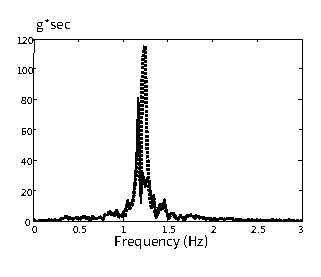
\includegraphics[width=0.25\textwidth] {figure/3-7a.eps}
   \label{fig:3-7a}
 }
 \subfigure[Hachinohe]{
   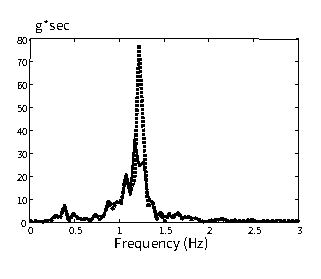
\includegraphics[width=0.25\textwidth] {figure/3-7b.eps}
   \label{fig:3-7b}
 }\\
 \subfigure[Mexico city]{
   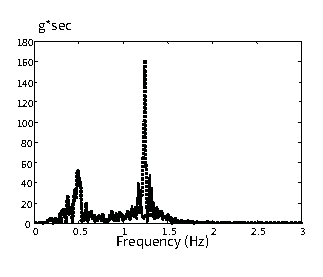
\includegraphics[width=0.25\textwidth] {figure/3-7c.eps}
   \label{fig:3-7c}
 }
 \subfigure[Northridge]{
   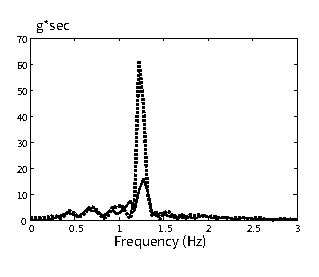
\includegraphics[width=0.25\textwidth] {figure/3-7d.eps}
   \label{fig:3-7d}
 }
%\caption{Structural acceleration in the time domain measured from the conventional shaking table test of TLD-structure interaction system (dotted line : without control, solid line : with control)}
\label{fig:3-6}
\end{figure}
dotted line : without control, solid line : with control
\end{frame}



\begin{frame}{Hybrid Testing for the Performance Evaluation of a TLD}
\begin{figure}[!ht]
\centering
 \subfigure[El Centro]{
   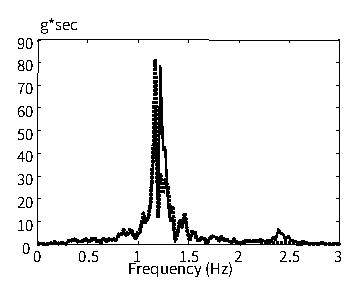
\includegraphics[width=0.25\textwidth] {figure/3-9a.eps}
   \label{fig:3-9a}
 }
 \subfigure[Hachinohe]{
   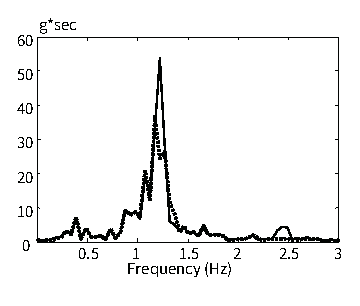
\includegraphics[width=0.25\textwidth] {figure/3-9b.eps}
   \label{fig:3-9b}
 }\\
 \subfigure[Mexico city]{
   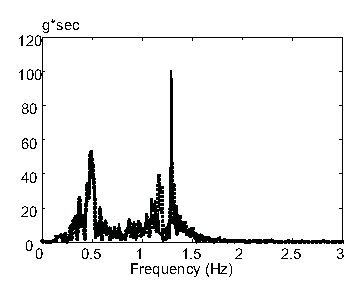
\includegraphics[width=0.25\textwidth] {figure/3-9c.eps}
   \label{fig:3-9c}
 }
 \subfigure[Northridge]{
   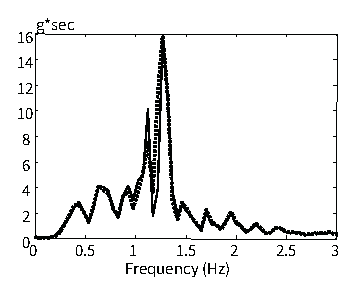
\includegraphics[width=0.25\textwidth] {figure/3-9d.eps}
   \label{fig:3-9d}
 }
\label{fig:3-9}
\end{figure}
dotted line : conventional shaking table test, solid line : real-time hybrid test
\end{frame}











\begin{frame}{Hybrid Testing for the Performance Evaluation of a TLCD}
\begin{figure}[ht]
\centering
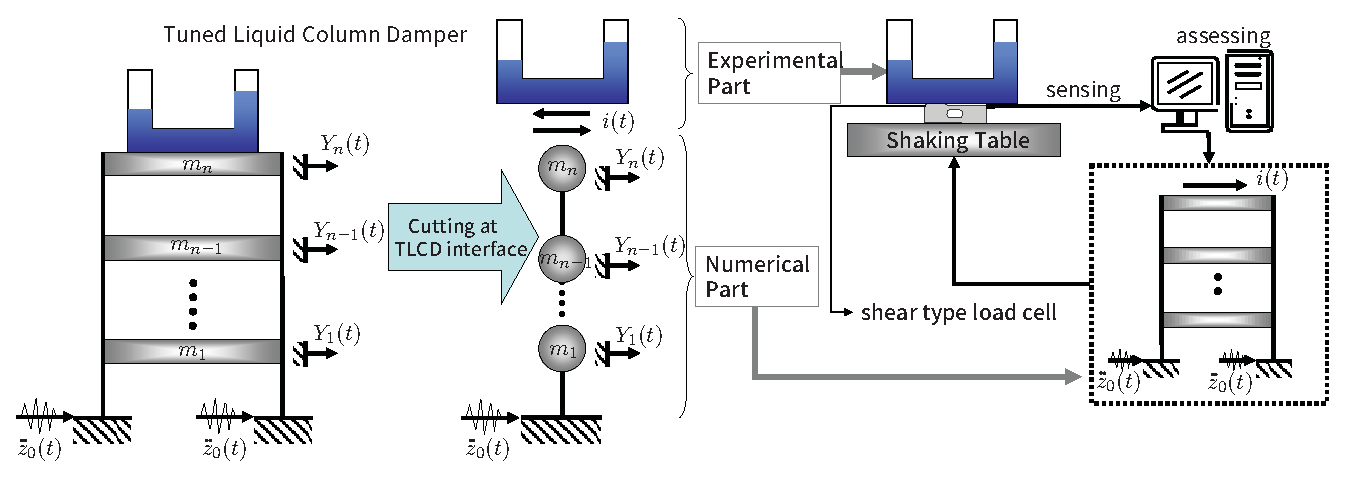
\includegraphics[width=1\textwidth] {figure/4-1.eps}
%\caption{Concept of the real-time hybrid testing method (TLCD)}
\label{fig:4-1}
\end{figure}
\end{frame}

\begin{frame}{Hybrid Testing for the Performance Evaluation of a TLCD}
\begin{figure}[ht]
\centering
\setcounter{subfigure}{0}
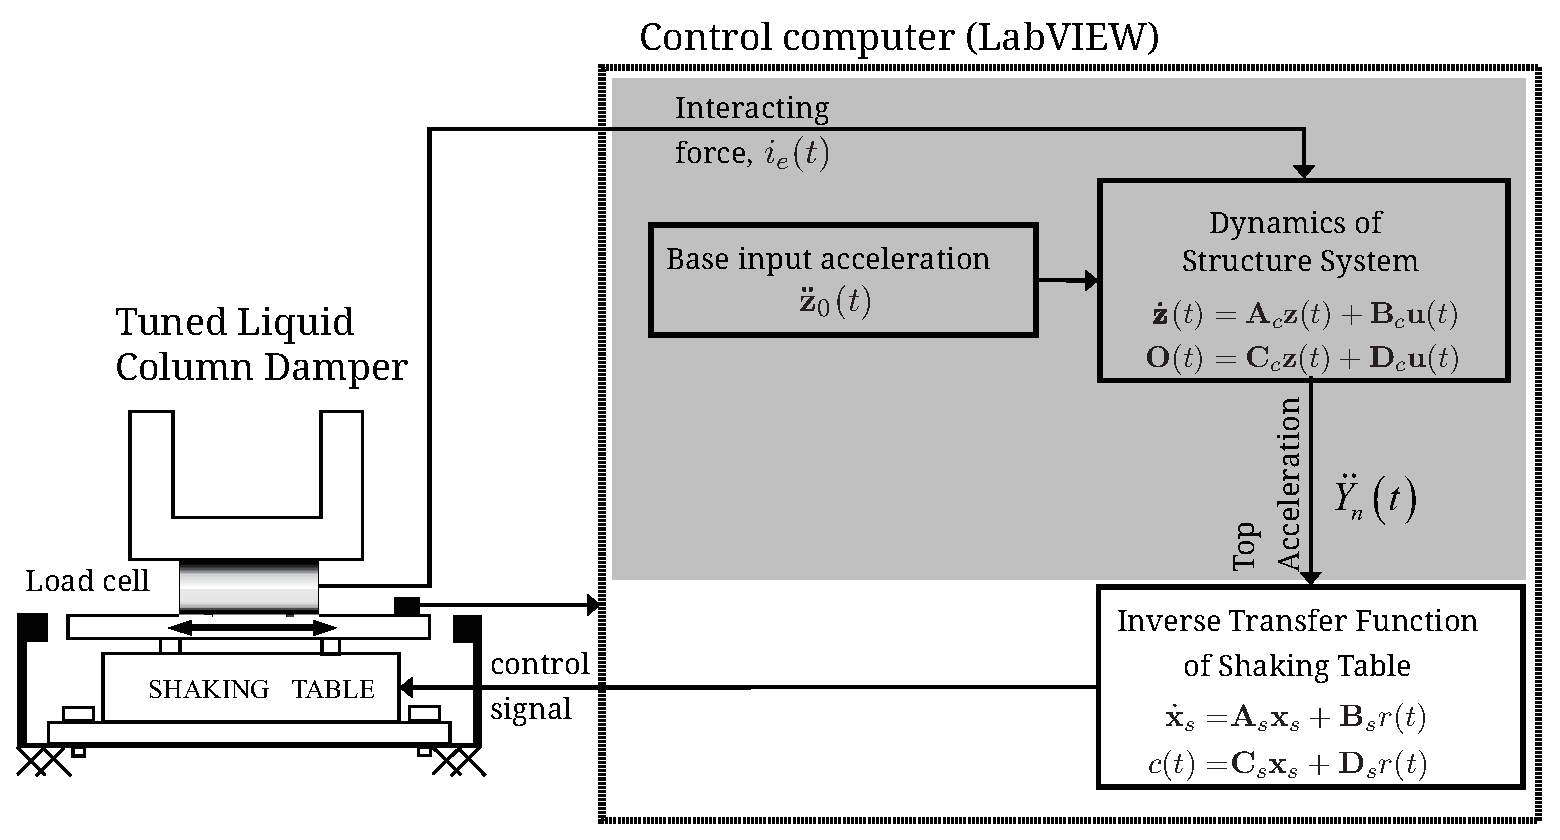
\includegraphics[width=1\textwidth] {figure/4-3.eps}
%\caption{Controller for implementing the real-time hybrid testing method}
\label{fig:4-3}
\end{figure}
\end{frame}

\begin{frame}{Hybrid Testing for the Performance Evaluation of a TLCD}
\begin{figure}[!ht]
\centering
\setcounter{subfigure}{0}
\subfigure[conventional testing method]{
   \includegraphics[width=0.4\textwidth] {figure/4-4a.eps}
   \label{fig:4-4a}
 }
 \subfigure[hybrid testing method]{
   \includegraphics[width=0.4\textwidth] {figure/4-4b.eps}
   \label{fig:4-4b}
 }
%\caption{Experimental view of a building with a TLCD}
\label{fig:4-4}
\end{figure}
\end{frame}

\begin{frame}{Hybrid Testing for the Performance Evaluation of a TLCD}
\begin{figure}[!ht]
\centering
\setcounter{subfigure}{0}
 \subfigure[El Centro Earthquake(time domain)]{
   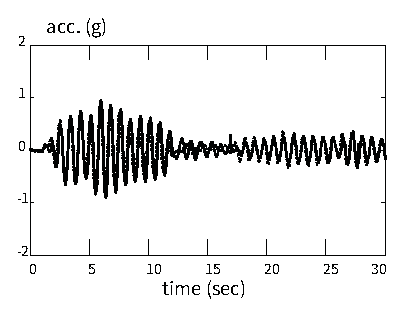
\includegraphics[width=0.3\textwidth] {figure/4-5a.eps}
   \label{fig:4-5a}
 }
 \subfigure[El Centro Earthquake(frequency domain)]{
   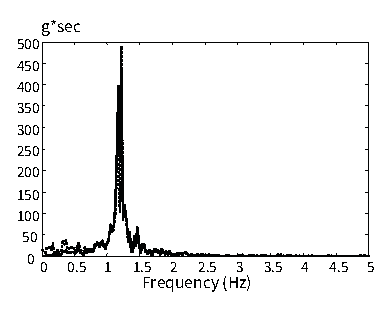
\includegraphics[width=0.3\textwidth] {figure/4-5b.eps}
   \label{fig:4-5b}
 }\\
 \subfigure[Kobe Earthquake(time domain)]{
   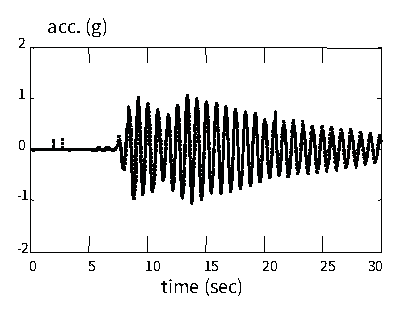
\includegraphics[width=0.3\textwidth] {figure/4-5c.eps}
   \label{fig:4-5c}
 }
 \subfigure[Kobe Earthquake(frequency domain)]{
   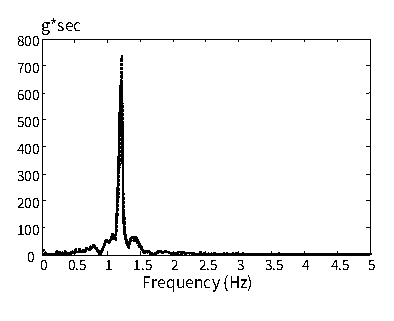
\includegraphics[width=0.3\textwidth] {figure/4-5d.eps}
   \label{fig:4-5d}
 }
\end{figure}
\end{frame}

\begin{frame}{Hybrid Testing for the Performance Evaluation of a TLMD}
\begin{figure}[ht]
\centering
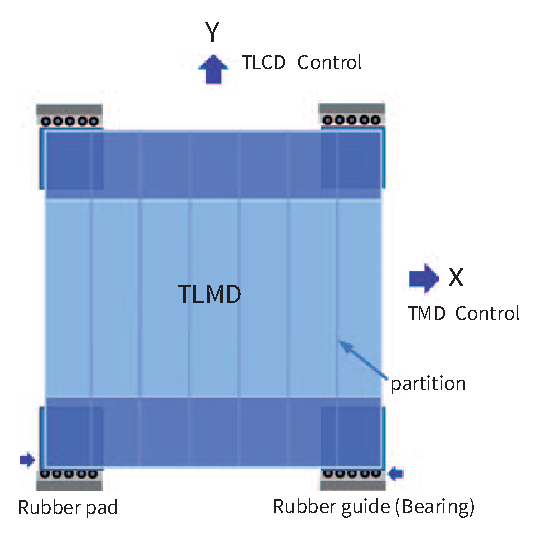
\includegraphics[width=0.6\textwidth] {figure/5-1.eps}
%\caption{Concept of a TLMD}
\label{fig:5-1}
\end{figure}
\end{frame}

\begin{frame}{Hybrid Testing for the Performance Evaluation of a TLMD}
\begin{figure}[ht]
\centering
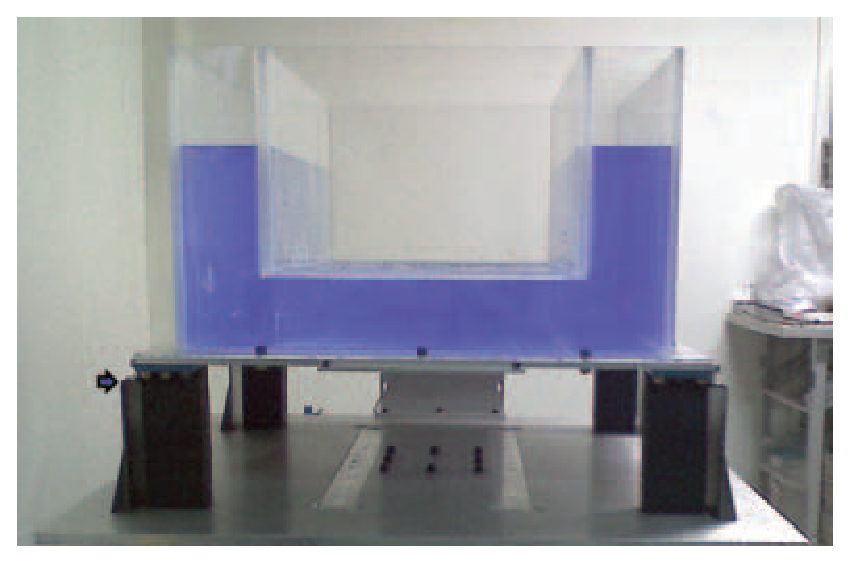
\includegraphics[width=0.6\textwidth] {figure/5-2.eps}
%\caption{Photograph of the manufactured TLMD}
\label{fig:5-2}
\end{figure}
\Fontvi
\begin{table}[ht]
\centering
\begin{tabularx}{\textwidth}{@{}X|X|X@{}}
\toprule[1pt]\midrule[0.3pt]
Design parameter & TLCD control direction & TMD control direction\\ \hline
Siffness or liquid length & $0.98m$ (liquid length) & $1990N/m$ (stiffness)\\
Frequency (Hz) & $0.73$ & $0.82$\\
Mass (kg) & $35$ & $75$\\
\bottomrule
\end{tabularx}
\caption{Design parameters of a TLMD model}
\label{tab:5-3}
\end{table}
\end{frame}


\begin{frame}{Hybrid Testing for a TLMD with a Building Structure}
\begin{figure}[ht]
\centering
\setcounter{subfigure}{0}
\subfigure[Design of the controller]{
   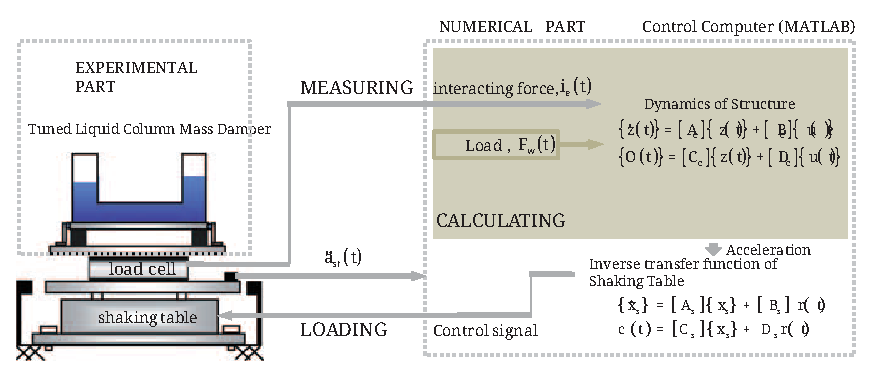
\includegraphics[width=0.7\textwidth] {figure/5-16.eps}
}
\subfigure[MATLAB Simulink window Target]{
   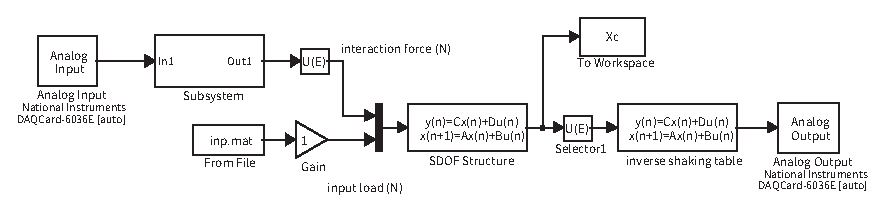
\includegraphics[width=0.7\textwidth] {figure/5-18.eps}
}
\end{figure}
\end{frame}


\begin{frame}{Hybrid Testing for a TLMD with a Building Structure}
\begin{figure}[!ht]
\centering
\setcounter{subfigure}{0}
\subfigure[Disp. TMD dir.]{
   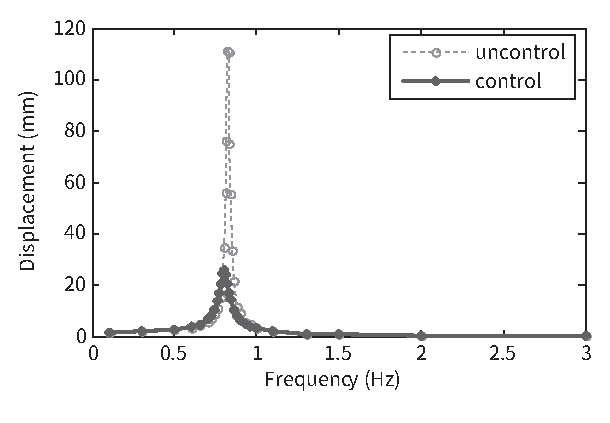
\includegraphics[width=0.3\textwidth] {figure/5-19.eps}
}
\subfigure[Acc. TMD dir.]{
   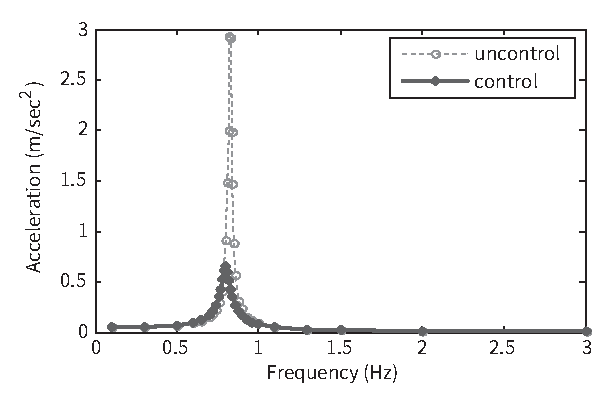
\includegraphics[width=0.3\textwidth] {figure/5-20.eps}
}
\subfigure[Disp. TMD dir.]{
   \includegraphics[width=0.3\textwidth] {figure/5-21.eps}
}
\subfigure[Disp. TLCD dir.]{
   \includegraphics[width=0.3\textwidth] {figure/5-22.eps}
}
\subfigure[Acc. TLCD dir.]{
   \includegraphics[width=0.3\textwidth] {figure/5-23.eps}
}
\subfigure[Disp. TLCD dir.t]{
   \includegraphics[width=0.3\textwidth] {figure/5-24.eps}
}
\end{figure}
\end{frame}

\section{Design of Controller}

\begin{frame}{Design of an Actuator for Simulating Wind Response}
\begin{figure}[!ht]
\centering
\includegraphics[width=0.8\textwidth] {figure/si.eps}
\end{figure}
\end{frame}

\begin{frame}{Design of an Actuator for Simulating Wind Response}
\begin{figure}[ht]
\centering
\includegraphics[width=0.8\textwidth] {figure/6-1.eps}
%\caption{Scheme of simulation of wind induced responses using LMS and ATMD}
\label{fig:6-1}
\end{figure}
Scheme of simulation of wind induced responses using LMS and ATMD
\end{frame}

\begin{frame}{Design of an Actuator for Simulating Wind Response}
Force of actuator
\begin{equation}
\begin{aligned}
\dot{\matr{z}} &=\matr{A}\matr{z}+\matr{B}_{f}f + \matr{B}_{u}u \\
y &= \matr{C}\matr{z}+\matr{D}_{f}f+\matr{D}_{u}u
\end{aligned}
\label{eq:6-1}
\end{equation}

\begin{equation}
\begin{aligned}
\matr{T}_{yf} &= \matr{Y}_{f}(s)\matr{F}(s)^{-1} = \matr{C}\left(s\matr{I}-\matr{A}\right)^{-1}\matr{B}_{f} \\
\matr{T}_{yu} &= \matr{Y}_{u}(s)\matr{U}(s)^{-1} = \matr{C}\left(s\matr{I}-\matr{A}\right)^{-1}\matr{B}_{u} \\
\end{aligned}
\label{eq:6-2}
\end{equation}

\begin{equation}
\begin{aligned}
\hat{\matr{U}}(s)&=\hat{\matr{T}}_{yu}^{-1}\hat{\matr{Y}}_{u}(s)\\
&=\hat{\matr{T}}_{yu}^{-1}\hat{\matr{Y}}_{f}(s)\\
&=\hat{\matr{T}}_{yu}^{-1}\hat{\matr{T}}_{yf}F(s)
\end{aligned}
\label{eq:6-4}
\end{equation}

\end{frame}


\begin{frame}{Design of an Actuator for Simulating Wind Response}
Filter and evelop function
\begin{equation}\label{eq:6-5}
\hat{\matr{U}}_{p}(\omega) = G(\omega)\hat{\matr{U}}(s)
\end{equation}

where,
\begin{align}
G(\omega) &= \frac{1-a_{co}}{2}cos \left( \frac{2\pi}{\omega_{2}-\omega_{1}}\omega \right) + \frac{1+a_{co}}{2}\label{eq:6-6}\\
a_{co} &=\left\{\begin{array}{lr} \omega < \omega_{1} &: 1 \\ \omega_{1} \leq \omega \leq \omega_{2} &: 0 \\ \omega > \omega_{2} &: 1\end{array} \right.
\label{eq:6-7}
\end{align}
\end{frame}

\begin{frame}{Design of an Actuator for Simulating Wind Response}
\begin{figure}[!ht]
\centering
\setcounter{subfigure}{0}
\subfigure[The shape of the band-stop filter]{
   \includegraphics[width=0.45\textwidth] {figure/6-2a.eps}
   \label{fig:6-2a}
 }
 \subfigure[The shape of the envelop function]{
   \includegraphics[width=0.45\textwidth] {figure/6-2b.eps}
   \label{fig:6-2b}
 }
%\caption{Exciter gain shape of the band-stop filter and the envelop function.}
\label{fig:6-2}
Exciter gain shape of the band-stop filter and the envelop function.
\end{figure}
\end{frame}

\begin{frame}{Design of an Actuator for Simulating Wind Response}
\begin{figure}[!ht]
\centering
\subfigure[Plan View of the 76-Story Building]{
   \includegraphics[width=0.3\textwidth] {figure/6-3a.eps}
   \label{fig:6-3a}\hfill
 }
 \subfigure[Elevation View of the Building.]{
   \includegraphics[width=0.3\textwidth] {figure/6-3b.eps}
   \label{fig:6-3b}
 }
\subfigure[Mode shapes of the Building.]{
   \includegraphics[width=0.3\textwidth] {figure/6-3c.eps}
   \label{fig:6-3c}\hfill
 }

%\caption{76th story benchmark model.}
\label{fig:6-3}
\end{figure}
76th story benchmark model.
\end{frame}

\begin{frame}{Design of an Actuator for Simulating Wind Response}
\begin{figure}[!ht]
\centering
\setcounter{subfigure}{0}
\subfigure[76th story acceleration response]{
   \includegraphics[width=0.8\textwidth] {figure/6-8a.eps}
   \label{fig:6-8a}\hfill
 }
 \subfigure[76th story displacement response]{
   \includegraphics[width=0.8\textwidth] {figure/6-8b.eps}
   \label{fig:6-8b}
 }

%\caption{Wind and LMS induced acceleration responses (when the target is 75th floor acceleration).}
\label{fig:6-8}
\end{figure}
Wind and LMS induced acceleration responses (when the target is 75th floor acceleration).
\end{frame}


\begin{frame}{Design of an Actuator for Simulating Wind Response}
\begin{figure}[!ht]
\centering
\setcounter{subfigure}{0}

 \subfigure[50th story acceleration response]{
   \includegraphics[width=0.8\textwidth] {figure/6-8c.eps}
   \label{fig:6-8c}\hfill
 }
 \subfigure[50th story displacement response]{
   \includegraphics[width=0.8\textwidth] {figure/6-8d.eps}
   \label{fig:6-8d}
 }

%\caption{Wind and LMS induced acceleration responses (when the target is 75th floor acceleration).}
\label{fig:6-8}
\end{figure}
Wind and LMS induced acceleration responses (when the target is 75th floor acceleration).
\end{frame}



\begin{frame}{Design of an Actuator for Simulating Wind Response}
\begin{figure}[!ht]
\centering
\setcounter{subfigure}{0}
 \subfigure[30th story acceleration response]{
   \includegraphics[width=0.8\textwidth] {figure/6-8e.eps}
   \label{fig:6-8e}\hfill
 }
 \subfigure[30th story displacement response]{
   \includegraphics[width=0.8\textwidth] {figure/6-8f.eps}
   \label{fig:6-8f}
 }
%\caption{Wind and LMS induced acceleration responses (when the target is 75th floor acceleration).}
\label{fig:6-8}
\end{figure}
Wind and LMS induced acceleration responses (when the target is 75th floor acceleration).
\end{frame}



\begin{frame}{Design of an Actuator for Simulating Wind Response}
ATMD Excitation
\begin{equation}\label{eq:6-10}
\matr{M}\matr{\ddot{x}}+\matr{C}\matr{\dot{x}}+\matr{K}\matr{x}+\matr{H}u = \eta\matr{W}
\end{equation}
Equation of motion of the building 
\begin{equation}\label{eq:6-11}
\begin{aligned}
\begin{bmatrix}\matr{M}_{s} & 0 \\ \matr{0} & m_{t}\end{bmatrix}
\begin{psmatrix}\matr{\ddot{x}}_{s} \\ \ddot{x}_{t}\end{psmatrix}+&
\begin{bmatrix}\matr{C}_{s}+c_{t}\matr{B}_{t}\matr{B}_{t}^{\top} & -c_{t}\matr{B}_{t} \\ -c_{t}\matr{B}_{t}^{\top} & c_{t}\end{bmatrix}
\begin{psmatrix}\matr{\dot{x}}_{s} \\ \dot{x}_{t}\end{psmatrix}+\\
&\begin{bmatrix}\matr{K}_{s}+k_{t}\matr{B}_{t}\matr{B}_{t}^{\top} & -k_{t}\matr{B}_{t} \\ -k_{t}\matr{B}_{t}^{\top} & k_{t}\end{bmatrix}
\begin{psmatrix}\matr{x}_{s} \\ x_{t}\end{psmatrix}  =
\begin{bmatrix}-\matr{B}_{t}\\1 \end{bmatrix}u
\end{aligned}
\end{equation}

\end{frame}


\begin{frame}{Design of an Actuator for Simulating Wind Response}
\begin{figure}[!ht]
\centering
\setcounter{subfigure}{0}
\subfigure[Transfer function of ATMD induced structure]{
   \includegraphics[width=0.45\textwidth] {figure/6-10a.eps}
   \label{fig:6-10a}\hfill
 }
 \subfigure[Frequency response of ATMD acceleration]{
   \includegraphics[width=0.45\textwidth] {figure/6-10b.eps}
   \label{fig:6-10b}
 }
 \subfigure[Frequency response of ATMD actuator force]{
   \includegraphics[width=0.45\textwidth] {figure/6-10c.eps}
   \label{fig:6-10c}\hfill
 }
 \subfigure[Time history of ATMD actuator force]{
   \includegraphics[width=0.45\textwidth] {figure/6-10d.eps}
   \label{fig:6-10d}
 }
%\caption{ATMD Excitation.}
\label{fig:6-10}
\end{figure}
\centering ATMD Excitation.
\end{frame}

\begin{frame}{Design of an Actuator for Simulating Wind Response}
\begin{figure}[!ht]
\centering
\setcounter{subfigure}{0}
\subfigure[76th story acceleration response]{
   \includegraphics[width=0.8\textwidth] {figure/6-11a.eps}
   \label{fig:6-11a}\hfill
 }
 \subfigure[76th story displacement response]{
   \includegraphics[width=0.8\textwidth] {figure/6-11b.eps}
   \label{fig:6-11b}
 }

%\caption{Wind and ATMD induced acceleration responses (when the target is 75th floor acceleration).}
\label{fig:6-11}
\end{figure}
Wind and ATMD induced acceleration responses (when the target is 75th floor acceleration).
\end{frame}

\begin{frame}{Design of an Actuator for Simulating Wind Response}
\begin{figure}[!ht]
\centering
\setcounter{subfigure}{0}

 \subfigure[50th story acceleration response]{
   \includegraphics[width=0.8\textwidth] {figure/6-11c.eps}
   \label{fig:6-11c}\hfill
 }
 \subfigure[50th story displacement response]{
   \includegraphics[width=0.8\textwidth] {figure/6-11d.eps}
   \label{fig:6-11d}
 }

%\caption{Wind and ATMD induced acceleration responses (when the target is 75th floor acceleration).}
\label{fig:6-11}
\end{figure}
Wind and ATMD induced acceleration responses (when the target is 75th floor acceleration).
\end{frame}



\begin{frame}{Design of an Actuator for Simulating Wind Response}
\begin{figure}[!ht]
\centering
\setcounter{subfigure}{0}

 \subfigure[30th story acceleration response]{
   \includegraphics[width=0.8\textwidth] {figure/6-11e.eps}
   \label{fig:6-11e}\hfill
 }
 \subfigure[30th story displacement response]{
   \includegraphics[width=0.8\textwidth] {figure/6-11f.eps}
   \label{fig:6-11f}
 }
%\caption{Wind and ATMD induced acceleration responses (when the target is 75th floor acceleration).}
\label{fig:6-11}
\end{figure}
Wind and ATMD induced acceleration responses (when the target is 75th floor acceleration).
\end{frame}



\begin{frame}{Pseudo-earthquake Testing of Real-scaled Building}
\begin{figure}[!ht]
\centering
\setcounter{subfigure}{0}
\subfigure[minor axis]{
   \includegraphics[width=0.18\textwidth] {figure/7-1a.eps}
   \label{fig:7-1a}\hfill
 }
 \subfigure[major axis]{
   \includegraphics[width=0.18\textwidth] {figure/7-1b.eps}
   \label{fig:7-1b}
 }
%\caption{Elevation view of the target structure.}
\label{fig:7-1}
\end{figure}
Elevation view of the target structure.
\end{frame}

\begin{frame}{Pseudo-earthquake Testing of Real-scaled Building}
\begin{figure}[ht]
\centering
\includegraphics[width=1\textwidth] {figure/7-3.eps}
%\caption{Schematic diagram of the field measurement, data acquisition and exciting system.}
\label{fig:7-3}
\end{figure}
Schematic diagram of the field measurement, data acquisition and exciting system.
\end{frame}

\begin{frame}{Pseudo-earthquake Testing of Real-scaled Building}
\begin{figure}[!ht]
\centering
\setcounter{subfigure}{0}
\subfigure[The measurement and data acquisition system]{
   \includegraphics[width=0.45\textwidth] {figure/7-4a.eps}
   \label{fig:7-4a}\hfill
 }
 \subfigure[The accelerometer installation]{
   \includegraphics[width=0.45\textwidth] {figure/7-4b.eps}
   \label{fig:7-4b}
 }
%\caption{Installation pictures of the measurement, data acquisition and exciting system.}
\label{fig:7-4}
\end{figure}
Installation pictures of the measurement, data acquisition and exciting system.
\end{frame}

\begin{frame}{Pseudo-earthquake Testing of Real-scaled Building}
\begin{figure}[ht]
\centering
\includegraphics[width=0.8\textwidth] {figure/7-5.eps}
%\caption{The transfer function from the absolute acceleration of the HMD to those of the structure.}
\label{fig:7-5}
\end{figure}
The transfer function from the absolute acceleration of the HMD to those of the structure.
\Fontvi
\begin{table}[ht]
\centering
\begin{tabularx}{\textwidth}{s|b|b}
\toprule[1pt]\midrule[0.3pt]
Modes & Frequency (Hz) \& COV (\%) & Damping ratio (\%) \& COV (\%)\\ \midrule[0.3pt]
1&0.52(1.82) & 1.46(14.42)\\
2&1.73(0.13) & 2.71(9.40)\\
3&2.94(0.10) & 3.54(1.93)\\
4&4.14(0.08) & 1.72(1.70)\\
5&5.36(0.23) & 3.84(3.56)\\
\bottomrule
\end{tabularx}
%\caption{Identified natural frequencies and damping ratios}
\label{tab:7-2}
\end{table}
Identified natural frequencies and damping ratios
\end{frame}

\begin{frame}{Forced Vibration Test of Real-scaled Building}
\begin{equation}\label{eq:7-4}
\matr{K}\Phi = \matr{M}_{a}\Phi\Lambda, \Phi^{\top}\matr{M}_{a}\Phi = \matr{I}
\end{equation}

\begin{equation}\label{eq:7-5}
\matr{K}^{\top} = \matr{K}
\end{equation}

\begin{equation}\label{eq:7-6}
J=\frac{1}{2}\left\| \matr{N}^{-1}\left(\matr{K}-\matr{K}_{a}\right)^{-1}\right\|
\end{equation}

\begin{equation}\label{eq:7-7}
\Phi = \Phi_{m} \left[ \Phi_{m}^{\top}\matr{M}_{a}\Phi_{m}\right]^{-1/2}
\end{equation}

\begin{equation}\label{eq:7-8}
\begin{aligned}
\matr{K}&=\matr{K}_{a} - \matr{K}_{a}\Phi\Phi^{\top}\matr{M}_{a}-\matr{M}_{a}\Phi\Phi^{\top}\matr{K}_{a}\\
&+\matr{M}_{a}\Phi\Phi^{\top}\matr{K}_{a}\Phi\Phi^{\top}\matr{M}_{a} + \matr{M}_{a}\Phi\Lambda\Phi^{\top}\matr{M}_{a}
\end{aligned}
\end{equation}
\end{frame}


\begin{frame}{Pseudo-earthquake Testing of Real-scaled Building}
\begin{figure}[!ht]
\centering
\setcounter{subfigure}{0}
\subfigure[1st mode shape]{
   \includegraphics[width=0.40\textwidth] {figure/7-6a.eps}
   \label{fig:7-6a}\hfill
 }
 \subfigure[2nd mode shape]{
   \includegraphics[width=0.40\textwidth] {figure/7-6b.eps}
   \label{fig:7-6b}
 }
%\caption{The mode shape comparison of initial, the measured and the updated FE models.}
\label{fig:7-6}
\end{figure}
The mode shape comparison of initial, the measured and the updated FE models.

\begin{table}[ht]
\centering
\begin{tabularx}{\textwidth}{@{}X|X|X|X|X|X@{}}
\toprule[1pt]\midrule[0.3pt]
& 1st mode & 2nd mode & 3rd mode & 4th mode & 5th mode\\ \midrule[0.3pt]
initial & 0.5022 & 1.5623 & 2.74 & 3.91 & 4.83\\
measured& 0.5249 & 1.7578 & 2.94 & 3.67 & 5.38\\
updated & 0.5249 & 1.7578 & 2.95 & 3.67 & 5.38\\
\bottomrule
\end{tabularx}
%\caption{Natural frequencies (Hz) for the modal testing tower}
\label{tab:7-3}
\end{table}
Natural frequencies (Hz) for the modal testing tower
\end{frame}


\begin{frame}{Pseudo-earthquake Testing of Real-scaled Building}
\begin{equation}\label{eq:7-11}
\begin{aligned}
\matr{\dot{z}}&= \matr{A}\matr{z} + \matr{B}_{b}\ddot{u}_{b}+\matr{B}_{h}\ddot{u}_{h}\\
\matr{y}&=\matr{C}\matr{z}+\matr{D}_{b}\ddot{u}_{b}+\matr{D}_{h}\ddot{u}_{h}
\end{aligned}
\end{equation}

\begin{equation}\label{eq:7-12}
\begin{aligned}
\matr{T}_{h}&=\matr{Y}_{h}(s)\matr{U}_{h}(s)^{-1} = \matr{C}\left(s\matr{I}-\matr{A}\right)^{-1}\matr{B}_{h} + \matr{D}_{h}\\
\matr{T}_{b}&=\matr{Y}_{b}(s)\matr{U}_{b}(s)^{-1} = \matr{C}\left(s\matr{I}-\matr{A}\right)^{-1}\matr{B}_{b}
\end{aligned}
\end{equation}

\begin{equation}\label{eq:7-13}
\matr{U}_{h}(s) = \matr{T}_{h}^{-1}\matr{Y}_{h}(s) = \matr{T}_{h}^{-1}\matr{Y}_{b}(s) = \matr{T}_{h}^{-1}\matr{T}_{b}\matr{U}_{b}(s)
\end{equation}

\begin{equation}\label{eq:7-14}
\hat{U}_{h}(s) = \hat{T}_{h}^{-1}\hat{Y}_{h}(s) = \hat{T}_{h}^{-1}\hat{Y}_{b}(s) = \hat{T}_{h}^{-1}\hat{T}_{b}\hat{U}_{b}(s)
\end{equation}

\end{frame}

\begin{frame}{Pseudo-earthquake Testing of Real-scaled Building}
\begin{figure}[!ht]
\centering
\setcounter{subfigure}{0}
\subfigure[Definition of the transfer function of the HMD]{
   \includegraphics[width=0.8\textwidth] {figure/7-9a.eps}
   \label{fig:7-9a}\hfill
 }
 \subfigure[Compensation the dynamics of HMD using the inverse transfer function]{
   \includegraphics[width=0.8\textwidth] {figure/7-9b.eps}
   \label{fig:7-9b}
 }
%\caption{Schematic diagram of the HMD controller.}
\label{fig:7-9}
\end{figure}
Schematic diagram of the HMD controller.
\end{frame}

\begin{frame}{Pseudo-earthquake Testing of Real-scaled Building}
\begin{figure}[!ht]
\centering
\setcounter{subfigure}{0}
\subfigure[1st floor acceleration]{
   \includegraphics[width=0.7\textwidth] {figure/7-12a.eps}
   \label{fig:7-12a}\hfill
}
\subfigure[2nd floor acceleration]{
   \includegraphics[width=0.7\textwidth] {figure/7-12b.eps}
   \label{fig:7-12b}
}
\subfigure[3rd floor acceleration]{
   \includegraphics[width=0.7\textwidth] {figure/7-12c.eps}
   \label{fig:7-12c}\hfill
}

%\caption{Time history comparison of El Centro earthquake response in the analysis and experimental models. (when the target response is the 5th floor acceleration).}

\end{figure}
Time history comparison of El Centro earthquake response in the analysis and experimental models. (when the target response is the 5th floor acceleration).
\end{frame}


\begin{frame}{Pseudo-earthquake Testing of Real-scaled Building}
\begin{figure}[!ht]
\centering
%\setcounter{subfigure}{0}
\subfigure[4th floor acceleration]{
   \includegraphics[width=0.7\textwidth] {figure/7-12d.eps}
   \label{fig:7-12d}
}
\subfigure[5th floor acceleration]{
   \includegraphics[width=0.7\textwidth] {figure/7-12e.eps}
   \label{fig:7-12e}\hfill
}
\subfigure[1st floor displacement]{
   \includegraphics[width=0.7\textwidth] {figure/7-12f.eps}
   \label{fig:7-12f}
}
%\caption{Time history comparison of El Centro earthquake response in the analysis and experimental models. (when the target response is the 5th floor acceleration).}

\end{figure}
Time history comparison of El Centro earthquake response in the analysis and experimental models. (when the target response is the 5th floor acceleration).
\end{frame}


\begin{frame}{Full scaled MR-damper}
\begin{figure}[!ht]
\centering
\subfigure[Components of full scaled MR Damper]{
   \includegraphics[width=0.4\textwidth] {figure/n3-6a.eps}
   \label{fig:n3-6a}\hfill
}
\subfigure[Manufactured full scaled MR Damper]{
   \includegraphics[width=0.4\textwidth] {figure/n3-6b.eps}
   \label{fig:n3-6b}
}

\label{fig:n3-6}
\end{figure}
\end{frame}

\begin{frame}{Full scaled MR-damper}
\begin{figure}[!ht]
\centering
\includegraphics[width=0.6\textwidth] {figure/n3-6c.eps}
   \label{fig:n3-6c}

\label{fig:n3-6}
\end{figure}
Manufactured MR damper with capcity of 1.0 ton
\end{frame}



\begin{frame}{Full state variable feedback for semi-active algorithms}

\begin{equation}\label{eq:n3-13}
P = \lim_{t\to\infty} E\left(\left[ \mathbf{x} - \hat{\mathbf{x}} \right] \left[ \mathbf{x} - \hat{\mathbf{x}} \right]^{\top}\right)
\end{equation}

\begin{equation}\label{eq:n3-14}
\begin{aligned}
\hat{\mathbf{x}} &= \left(\mathbf{A}-\mathbf{LC}\right)\hat{\mathbf{x}} + \begin{bmatrix}\mathbf{L} & \mathbf{B}-\mathbf{LD}\end{bmatrix} \begin{psmatrix}\mathbf{y}\\\mathbf{u}\end{psmatrix} \\
\begin{psmatrix}\hat{\mathbf{y}}\\\hat{\mathbf{x}}\end{psmatrix} & = \begin{bmatrix}\mathbf{C} \\ \mathbf{I}\end{bmatrix}\hat{\mathbf{x}} + \begin{bmatrix}\mathbf{0} & \mathbf{D}\\ \mathbf{0} & \mathbf{0}\end{bmatrix}\begin{psmatrix}y \\ \mathbf{u}\end{psmatrix}
\end{aligned}
\end{equation}

\end{frame}

\begin{frame}{MR Damper Test}
\begin{figure}[ht]
\centering
\subfigure[Installation of MR damper and load cell]{
\includegraphics[width=0.4\textwidth] {figure/installed1.eps}
}
\subfigure[LVDT type displacement sensor (Midori America LP-19FB)]{
\includegraphics[width=0.4\textwidth] {figure/installed2.eps}
}
\end{figure}
MR damper installation
\end{frame}




\begin{frame}{MR Damper Optimal Passive Controlled Result}
\begin{figure}[!ht]
\centering
\includegraphics[width=0.6\textwidth] {figure/n3-12.eps}

\label{fig:n3-12}
\end{figure}
Normalized maximum displacement of passive control cases (first floor).
\end{frame}

\begin{frame}{MR Damper Optimal Passive Controlled Result}
\begin{figure}[!ht]
\centering
\includegraphics[width=0.6\textwidth] {figure/n3-13.eps}
\label{fig:n3-13}
\end{figure}
Normalized maximum acceleration of passive control cases.
\end{frame}



\begin{frame}{MR Damper Semi-active controlled Result}
\begin{figure}[!ht]
\centering
\includegraphics[width=0.6\textwidth] {figure/n3-14.eps}
\label{fig:n3-14}
\end{figure}
Normalized maximum displacement comparison of MR damper-based control systems.
\end{frame}

\begin{frame}{MR Damper Semi-active controlled Result}
\begin{figure}[!ht]
\centering
\includegraphics[width=0.6\textwidth] {figure/n3-15.eps}
\label{fig:n3-15}
\end{figure}
Normalized maximum acceleration comparison of MR damper-based control systems.
\end{frame}


\begin{frame}{MR Damper Test Time-history Result}
\begin{figure}[!ht]
\centering
\includegraphics[width=0.5\textwidth] {figure/n3-16.eps}
\label{fig:n3-16}
\end{figure}
Time history responses of displacement at the first floor under the El Centro earthquake.
\end{frame}

\begin{frame}{MR Damper Test Time-history Result}
\begin{figure}[!ht]
\centering
\includegraphics[width=0.5\textwidth] {figure/n3-17.eps}
\end{figure}
Time history responses of acceleration at the second floor under the Kobe earthquake.
\label{fig:n3-17}
\end{frame}






\section{Hybrid Testing of Building with MR Damper}
%Real-time Hybrid Test on a Semi-actively Controlled Building Structure Equipped with Full-scale MR Dampers


\begin{frame}{Hybrid Testing of Building Structure with MR Damper}
\begin{figure}[!ht]
\centering
\setcounter{subfigure}{0}
\subfigure[structural control system]{
   \includegraphics[width=0.2\textwidth] {figure/8-1a.eps}
   \label{fig:8-1a}\hfill
 }
\subfigure[experimental and numerical substructures]{
   \includegraphics[width=0.4\textwidth] {figure/8-1b.eps}
   \label{fig:8-1b}
}
\subfigure[implementation of RT-HYTEM]{
   \includegraphics[width=0.5\textwidth] {figure/8-1c.eps}
   \label{fig:8-1c}
}
%\caption{Conceptual view of RT-HYTEM for a building with an MR damper.}
\label{fig:8-1}
\end{figure}
Conceptual view of the hybrid testing method for a building with an MR damper.
\end{frame}

\begin{frame}{Hybrid Testing of Building Structure with MR Damper}
\begin{figure}[!ht]
\centering
\includegraphics[width=0.45\textwidth] {figure/8-2.eps}
%\caption{Configuration of experimental system.}
\label{fig:8-2}
\end{figure}
Configuration of experimental system.
\end{frame}


\begin{frame}{Hybrid Testing of Building Structure with MR Damper}
\begin{figure}[ht]
\centering
\includegraphics[width=0.7\textwidth] {figure/8-3.eps}
%\caption{Schematic view of experimental set-up: (a) building model installed with an MR damper, (b) UTM installed MR damper, and (c) experimental instrumentation.}
\label{fig:8-3}
\end{figure}
Schematic view of experimental set-up: (a) building model installed with an MR damper, (b) UTM installed MR damper, and (c) experimental instrumentation
\end{frame}

\begin{frame}{Hybrid Testing of Building Structure with MR Damper}
\begin{figure}[H]
\centering
\includegraphics[width=0.7\textwidth] {figure/8-7.eps}
%\caption{Integrated controller for implementing RTHTM.}
\label{fig:8-7}
\end{figure}
Integrated controller for implementing the hybrid testing method.
\end{frame}

\begin{frame}{Hybrid Testing of Building Structure with MR Damper}
\begin{figure}[H]
\centering
\setcounter{subfigure}{0}
\subfigure[time history of force]{
   \includegraphics[width=0.9\textwidth] {figure/8-8a.eps}
   \label{fig:8-8a}
}
\subfigure[force-displacement relation]{
   \includegraphics[width=0.45\textwidth] {figure/8-8b.eps}
   \label{fig:8-8b}
}
\subfigure[force-velocity relation]{
   \includegraphics[width=0.42\textwidth] {figure/8-8c.eps}
   \label{fig:8-8c}
}
%\caption{Comparison between calculated and experimentally measured responses for the Bouc-Wen model.}
\label{fig:8-8}
\end{figure}
Comparison between calculated and experimentally measured responses for the Bouc-Wen model.
\end{frame}


\begin{frame}{Hybrid Testing of Building Structure with MR Damper}
\begin{figure}[H]
\centering
\setcounter{subfigure}{0}
\subfigure[absolute acceleration responses]{
   \includegraphics[width=0.8\textwidth] {figure/8-9a.eps}
   \label{fig:8-9a}
}
%\caption{Comparison between calculated and experimentally measured responses under El Centro earthquake excitation.}
\label{fig:8-9}
\end{figure}
Comparison between calculated and experimentally measured responses under El Centro earthquake excitation.
\end{frame}


\begin{frame}{Hybrid Testing of Building Structure with MR Damper}
\begin{figure}[H]
\centering
\subfigure[displacement responses]{
   \includegraphics[width=0.8\textwidth] {figure/8-9b.eps}
   \label{fig:8-9b}
}
%\caption{Comparison between calculated and experimentally measured responses under El Centro earthquake excitation.}
\label{fig:8-9}
\end{figure}
Comparison between calculated and experimentally measured responses under El Centro earthquake excitation.
\end{frame}


\begin{frame}{Hybrid Testing of Building Structure with MR Damper}
\begin{figure}[H]
\centering
\setcounter{subfigure}{0}
\subfigure[force-displacement relation]{
   \includegraphics[width=0.45\textwidth] {figure/8-13a.eps}
   \label{fig:8-13a}
}
\subfigure[force-velocity relation]{
   \includegraphics[width=0.45\textwidth] {figure/8-13b.eps}
   \label{fig:8-13b}
}\\

%\caption{Identified Bouc-Wen parameters and the numerical model of an MR damper.}
\label{fig:8-13}
\end{figure}
Identified Bouc-Wen parameters and the numerical model of an MR damper.
\end{frame}


\begin{frame}{Hybrid Testing of Building Structure with MR Damper}
\begin{figure}[H]
\centering
\setcounter{subfigure}{0}
\subfigure[shape parameter]{
   \includegraphics[width=0.3\textwidth] {figure/8-13c.eps}
   \label{fig:8-13c}
}
\subfigure[damping coefficient of an MR damper]{
   \includegraphics[width=0.3\textwidth] {figure/8-13d.eps}
   \label{fig:8-13d}
}
\subfigure[shape parameter $\alpha$]{
   \includegraphics[width=0.3\textwidth] {figure/8-13e.eps}
   \label{fig:8-13e}
}
%\caption{Identified Bouc-Wen parameters and the numerical model of an MR damper.}
\label{fig:8-13}
\end{figure}
Identified Bouc-Wen parameters and the numerical model of an MR damper.
\end{frame}



\begin{frame}{Hybrid Testing of Building Structure with MR Damper}
\begin{figure}[H]
\centering
\includegraphics[width=1\textwidth] {figure/8-14.eps}
%\caption{Clipped-optimal and RT-HYTEM integrated controller.}
\label{fig:8-14}
\end{figure}
Clipped-optimal algorithm and the hybrid test integrated controller.
\begin{equation}\label{eq:8-21}
v_{i} = V_{\text{max}}H\left(\left\{f_{c_{i}}-f_{i}\right\}f_{i}\right)
\end{equation}
\end{frame}


\begin{frame}{Hybrid Testing of Building Structure with MR Damper}
\begin{figure}[H]
\centering
\includegraphics[width=1\textwidth] {figure/8-15.eps}
%\caption{MHF and RT-HYTEM integrated controller.}
\label{fig:8-15}
\end{figure}
MHF algorithm and hybtid test integrated controller.
\begin{equation}\label{eq:8-22}
N_{i}(t)=g_{i}|P\left[\Delta_{i}(t)\right]|
\end{equation}
\begin{equation}\label{eq:8-23}
f_{n_{i}}=\mu g_{i}|P\left[\Delta_{i}(t)\right]=g_{n_{i}}|P\left[\Delta_{i}(t)\right]
\end{equation}
\begin{equation}\label{eq:8-24}
v_{i} = V_{\text{max}}H\left(f_{n_{i}}-|f_{i}|\right)
\end{equation}
\end{frame}

\begin{frame}{Hybrid Testing of Building Structure with MR Damper}
\begin{figure}[H]
\centering
\includegraphics[width=0.8\textwidth] {figure/8-16.eps}
%\caption{Experimental results, in the time domain under El Centro earthquake excitation at different applied currents.}
\label{fig:8-16}
\end{figure}
Experimental results, in the time domain under El Centro earthquake excitation at different applied currents
\end{frame}



\begin{frame}{Hybrid Testing of Building Structure with MR Damper}
\begin{figure}[H]
\centering
\includegraphics[width=0.8\textwidth] {figure/8-17.eps}
%\caption{Experimental results, in the time domain under Northridge earthquake excitation at different applied currents.}
\label{fig:8-17}
\end{figure}
Experimental results, in the time domain under Northridge earthquake excitation at different applied currents
\end{frame}

\begin{frame}{Hybrid Testing of Building Structure with MR Damper}
\begin{figure}[H]
\centering
\setcounter{subfigure}{0}
\subfigure[El Centro earthquake]{
   \includegraphics[width=0.4\textwidth] {figure/8-20a.eps}
   \label{fig:8-20a}
}
\subfigure[Kobe earthquake]{
   \includegraphics[width=0.4\textwidth] {figure/8-20b.eps}
   \label{fig:8-20b}
}
\subfigure[Northridge earthquake]{
   \includegraphics[width=0.6\textwidth] {figure/8-20c.eps}
   \label{fig:8-20c}
}
%\caption{Passive and semi-active RT-HYTEM experimental results(time domain).}
\label{fig:8-20}
\end{figure}
Passive and semi-active contolled results(time domain).
\end{frame}

\begin{frame}{Hybrid Testing of Building Structure with MR Damper}
\begin{figure}[H]
\setcounter{subfigure}{0}
\subfigure[El Centro earthquake]{
   \includegraphics[width=0.4\textwidth] {figure/8-21a.eps}
   \label{fig:8-21a}
}
\hfill\subfigure[Kobe earthquake]{
   \includegraphics[width=0.4\textwidth] {figure/8-21b.eps}
   \label{fig:8-21b}
}\\
\subfigure[Northridge earthquake]{
   \includegraphics[width=0.4\textwidth] {figure/8-21c.eps}
   \label{fig:8-21c}
}
\hfill\subfigure{
   \includegraphics[width=0.2\textwidth] {figure/8-21d.eps}
}
%\caption{Passive and semi-active RT-HYTEM experimental results(frequency domain).}
\label{fig:8-21}
\end{figure}
Passive and semi-active controlled results(frequency domain).
\end{frame}



\section{Conclusion}

\begin{frame}{Conclusion}
\begin{itemize}
   \item 하이브리드 실험법과 동적 응답을 구현하는 가진시스템 설계법을 제안
   \item 하이브리드 실험의 선행 연구로서 부분구조 실험법을 수행하였으며, TLD와 TLCD 그리고 새로운 형태의 2방향 제어장치 TLMD 하이브리드 실험과 일반적인 진동대 실험을 비교
   \item LMS와 ATMD를 사용하여 76층 벤치마크 건물의 풍하중 구현을 수치해석적으로 검증
   \item HMD를 사용하여 실물규모 5층 건물의 지진응답을 구현하는 실험을 수행
   \item 실물규모 5층 건물에 1톤급 MR감쇠기를 설치하고 수동 및 준능동 알고리즘을 적용 및 HMD를 사용하여 유사지진 하중 구현하여 내진 성능 실험을 수행
   \item 1톤급 실물크기의 MR감쇠기를 UTM에 장착하여 하이브리드 실험법으로 수동 제어 및 준능동 제어성능을 검증
\end{itemize}
\end{frame}



\begin{frame}{2차 심사 반영 사항 수정 사항}
\begin{itemize}
   \item RT-HYTEM, real-time 삭제.
   \item Hybrid testing method로 용어 통일 (김준희 교수님, 민경원 교수님 지적사항)
   \item 오타, 인용 수정, 약어 중복 표기 삭제, 중복된 내용 모두 삭제, 중복된 그림 및 수식 삭제
   \item 1장 Literature Review 수정, SCI논문의 서론에 쓰인 문구들 제거, 그림 캡션 내용 수정
   \item 3장 Exciting -> Excitation system 등으로 수정 (이상현 교수님 지적사항)
   \item 3장 Excitation과 Actuator의 중복표기 문제 : 제목 표기엔 Excitation으로 표기 내용중에 LMS와 ATMD를 통틀어 Actuator로 언급 (이성경 교수님 지적사항)
   \item 3장 HMD 가진 신호 데이터 추가 (Figure 3.34, Figure 3.35)
   \item 4장 Investigation -> Verification 으로 수정 (박지훈 교수님 지적사항)
   \item 결론 내용 수정
\end{itemize}
\end{frame}

\begin{frame}{2차 심사 반영 사항 수정 사항}
\begin{itemize}
   \item 초록 : 소개 -> 제안으로 수정 (박지훈 교수님 지적사항), 맞춤법 표기 수정
   \item Further study 삭제
   \item 논문 편집 : 그림, 표 위치 수정 (민경원 교수님 지적사항)
   \item CV 추가 : 연구실적과 이력내용 추가 (민경원 교수님 지적사항)
   \item Nonlinear damper (비선형 감쇠기)로 꼭 국한해야 하는지? (박지훈 교수님) : 하이브리드 실험법이 선형 구조계를 실험 중 수치해석으로 계산하기 때문에 실험부가 선형 거동할 경우 하이브리드 실험의 의미가 상쇄된다고 판단합니다. 하이브리드 실험을 수행하기에 앞서 선형거동이 예측되는 구조계와 그렇지 않은 구조계를 명확히 구분하고 비선형 감쇠기나 비선형 구조계로 실험체를 국한해야 실험의 의미가 있기 때문에 비선형 감쇠장치를 제목에 포함하는 것이 좋다고 생각합니다.
   \item 영문 문법, 표기 관련 교정 완료 (https://grammarly.com)
   \item 논문내용을 지속적으로 읽어가며 퇴고 중.
\end{itemize}
\end{frame}

\begin{frame}{Work Experience}
\begin{itemize}
   \item 초고층 건물의 GNSS 망조정기법과 외란보정 기법을 이용한 거푸집 연직도 관리 (건설신기술)
   \item 코레일 공항철도 및 KTX 진동가속도 분석 시스템
   \item LCD Display 글래스 이송로봇 사전감지시스템 (Early Warning System)
   \item 초고층건물 구조건전도 모니터링 Structural Health Monitoring
   \item 도로 안개 소산 시스템 프로젝트 (image processing)
   \item 지하철 역사 초기 재난 대응 M2M 대피경로 안내 시스템 (IoT, M2M)
   \item 코레일 KTX 콘크리트도상 상태평가 과제 (crack detection, computer vision)
   \item 코레일 재해우려개소 낙석감지 시스템 (computer vision)
   \item 코레일 승무원 검표지원 시스템 (computer vision)
\end{itemize}
\end{frame}

\end{document}
